% ---------------------------------------------------------------------
%                      DOCUMENTO DE EJEMPLO
%          QUE UTILIZA LA PLANTILLA DE LA EDITORIAL DE LA
%                UNIVERSITAT POLITÈCNICA DE VALÈNCIA
%                  PARA TRABAJOS DE FIN DE GRADO
%                         CAMPUS D'ALCOI
% ---------------------------------------------------------------------

\documentclass[tfg, rm, valencia]{tfgepsa}

% Opciones de la clase 'tfgepsa'
%
% tfg		  - Format TFG
% imprimir    - Doble cara márgenes horizontales asimétricos (parar imprimir)
% ebookpdf    - Formato PDF para tabletas
% rm          - Tipo de letra roman
% sf          - Tipo de letra sanserif
%
% nomathskip  - No se modifican las distancias de las ecuaciones 
%
% castellano  - El TFG está escrito en castellano
% valencia    - El TFG està escrit en valencià
% english     - El TFG está escrito en inglés

% ---------------------------------------------------------------------
% Configuraciones presonalizadas 

% ---------------------------------------------------------------------
% ---------------------------------------------------------------------
% Configuración general

\usepackage[utf8]{inputenc}
\usepackage[T1]{fontenc}

\ifcastellano\usepackage[spanish,es-tabla]{babel}\fi
\ifvalencia\usepackage[catalan]{babel}\fi
\ifenglish\usepackage[english]{babel}\usepackage{csquotes}\fi
\newcommand{\sen}{\on{sen}}	

\usepackage{xcolor}
\usepackage{array,booktabs}
\usepackage{tabularx,longtable,multicol,multirow}
\usepackage{subcaption}
\usepackage{amsmath}
\usepackage{amssymb}

%\ifenglish
%	\raggedright % No justifica, i no divide las palabras con guiones
%\fi

% ---------------------------------------------------------------------
% ---------------------------------------------------------------------
% Bibliografía

\usepackage[
	url = false,
	style = numeric,
	hyperref = true,
	backref = true,
	backend = biber, % Otra opción es 'backend = bibtex'
	%backend = bibtex,
	]{biblatex}

% ---------------------------------------------------------------------
% ---------------------------------------------------------------------
% Documento electrónico

\usepackage{makeidx}
\makeindex

\ifEBOOKPDF
	\colorlet{colorEnlace}{red!75!black} 
\else
    \ifImprimir
	    \colorlet{colorEnlace}{black} 
    \else
        \colorlet{colorEnlace}{blue!85!black} 
    \fi
\fi

\usepackage[
	{colorlinks},
	{linkcolor=colorEnlace},
	{citecolor=colorEnlace},
	{urlcolor=colorEnlace},
	{bookmarksnumbered},
	{breaklinks},
	]{hyperref}

% ---------------------------------------------------------------------
% ---------------------------------------------------------------------
% Expresión de unidades según el Sistema Internacional, monedas

\usepackage{eurosym}
\usepackage{siunitx}

\ifenglish
	\sisetup{output-decimal-marker={.}}
\else
	\sisetup{output-decimal-marker={,}}
\fi

\DeclareSIUnit[number-unit-product = {\;}] \EURO{\geneuro}

% ---------------------------------------------------------------------

\newcommand{\ingles}[1]{\textit{#1}}
\newenvironment{ParrafoIngles}{\itshape}{}

% ------------------------------------------------------------------------

\usepackage{xspace}

\newcommand{\angles}[1]{\textit{#1}\/}
\newcommand{\miUrl}[1]{{\small%
	%\texttt%
	{\underline{#1}}}}

\newcommand{\matlabr}{{\sc Matlab}$^\circledR$\xspace}
\newcommand{\simulinkr}{\textit{Simulink}$^\circledR$\xspace}
\newcommand{\matlab}{{\textsc{Matlab}}\xspace}
\newcommand{\simulink}{\textit{Simulink}\xspace}

\newcommand{\scr}{\textit{script\/}\xspace}
\newcommand{\scrs}{\textit{scripts\/}\xspace}

% ------------------------------------------------------------------------

\definecolor{griset}{rgb}{.925, .925, .925}

\newsavebox{\mybox}
\newenvironment{parrafoDestacado}
	{%
	\fboxsep = 2ex
	\fboxrule = .4pt
  	\begin{lrbox}{\mybox}%
  	\begin{minipage}{.85\textwidth-2\fboxsep}\itshape\parskip=2ex
	}
	{%
	\end{minipage}
  	\end{lrbox}%
	\begin{flushright}
		\colorbox{griset}{\usebox{\mybox}}%
  		%\fcolorbox{black}{griset}{\usebox{\mybox}}%
	\end{flushright}
	}

% ------------------------------------------------------------------------
% Resumen del capítulo

\newsavebox{\myboxb}
\newenvironment{Resumen}
	{%
	\vspace*{-2.0cm}
	\fboxsep = 0pt
	\fboxrule = 0pt
  	\begin{lrbox}{\myboxb}%
  	\begin{minipage}{.85\textwidth}\itshape\parskip=2ex\parindent=2em
	}
	{%
	\end{minipage}
  	\end{lrbox}%
	\begin{flushright}
		\usebox{\myboxb}%
	\end{flushright}
	\vspace{0.5cm}
	}

% ---------------------------------------------------------------------
% ---------------------------------------------------------------------
% Símbolos matemáticos

\newcommand{\on}{\operatorname}
\usepackage{amsmath}
\DeclareMathOperator*{\argmax}{argmax}
\DeclareMathOperator*{\argmin}{argmin}

% ---------------------------------------------------------------------
% ---------------------------------------------------------------------
% Teoremas y ejemplos

\ifcastellano
	\newtheorem{teorema}{\upshape\bfseries Teorema}[section]
	\newtheorem{lema}{\mdseries\scshape Lema}[section]
	\newtheorem{proposicion}{\upshape\bfseries Proposición}[section]
	\newtheorem{ejemplo}{\bfseries\scshape Ejemplo}[section]
\fi

\ifvalencia % Es mantenen els mateixos noms per compatibilitat, però l'autor els pot personalitzar
	\newtheorem{teorema}{\upshape\bfseries Teorema}[section]
	\newtheorem{lema}{\mdseries\scshape Lema}[section]
	\newtheorem{proposicion}{\upshape\bfseries Proposició}[section]
	\newtheorem{ejemplo}{\bfseries\scshape Exemple}[section]
\fi

\ifenglish
	\newtheorem{teorema}{\upshape\bfseries Theorem}[section]
	\newtheorem{lema}{\mdseries\scshape Lemma}[section]
	\newtheorem{proposicion}{\upshape\bfseries Proposition}[section]
	\newtheorem{ejemplo}{\bfseries\scshape Example}[section]
\fi

% ---------------------------------------------------------------------


\usepackage{listings}

% \lstset{deletekeywords=[1]{structure}}

\lstset{
	language=[LaTeX]TeX,
	basicstyle=\fontsize{10.5pt}{12.5pt}\selectfont\ttfamily,         
	identifierstyle=,           
	commentstyle=\color[rgb]{.5,.5,.5},
	stringstyle=\color[rgb]{0,.5,0},
	tabsize=4,
	backgroundcolor = \color[rgb]{.96,.96,.96},
	rulecolor = \color[rgb]{.96,.96,.96},
	frame=single,
	framesep = 9pt,
	xleftmargin= 9pt,
	xrightmargin= 9pt,			
	classoffset=0,
	morekeywords={
		comando, marcaseccion, href,
		maketitle,
		signature, address, opening, closing, encl,
		appendix, include, includeonly, input,
		titlelabel, titleformat, thetitle, titlecontents, thecontentslabel, phantomsection, 
		addstarredchapter,
		nameref, indexIngles, printindex, 
		contentspage, titlerule, tableofcontents,
		dominitoc, minitoc,
		citet, citep, citeauthor, citeyear,
		sffamily, Large, familydefault, sfdefault,
		geometry, newgeometry, restoregeometry,
		autoref, nouppercase,
		tablename, figurename,contentsname,chaptername, bibname,
		colorlet,
		columncolor, rowcolor, ctable, LL, FL, ML, NN,
		toprule, midrule, cmidrule, arraybackslash, bottomrule, newcolumntype,
		chaptermark, thechapter,
		anchoPapel, margenInterior, ingles, comandoNuevo, SAC, SACs, todoDestacado, todoNormal,
		xspace, destacado, espacio, longLinea,
		labelitemi, labelitemii, labelitemiii, labelitemiv,
		labelenumi, labelenumii, labelenumiii, labelenumiv,
		mathcal,
		listoftables, listoffigures,
		columnbreak, clearpage,
		graphicspath, totalnumber, rotatebox, scalebox, resizebox, captionfo, subfloat,
		bottomnumber, topnumber,
		fbox, framebox, fcolorbox, colorbox, shadowbox, doublebox, ovalbox, Ovalbox, shadowsize,
		cornersize,
		setlength, floatstyle, newfloat, floatname, endfoot, endlastfood, endhead, endfirsthead,
		dfrac, tfrac, sen, tg, dif, overset, underset, text, eqref, nolimits,
		numberwithin, SI, si, num, euro, EURO, finEjemplo,
		pascal, kelvin, kilo, metre, meter, square, percent, kilogram, kilometre, per, second, hour, newton, volt, micro, centi, Picture,
		theoremstyle, theoremheaderfont, theorembodyfont,
		includeonlyframes, frametitle, framesubtitle, mode, usetheme, usecolortheme, usefonttheme,
		useinnertheme, useoutertheme, note, setbeameroption, pgfpagesuselayout, pause, alert,
		structure, only, onslide, visible, invisible, uncover, alt, temporal, column, setlist,
		ifEBOOKPDF, ifenglish, encabezadoPaginaImpar, Titulo, Alumnoa, Tutores, Titulacion, Convocatoria		
		},
	keywordstyle=\color[rgb]{.45,.00,.00},
	classoffset=1,
	morekeywords={
		begin,
		end,
		chapter, section, subsection, part, includegraphics,
		chapter*, section*, subsection*,
		subsubsection, paragraph, subparagraph,
		},
	keywordstyle=\color{blue},
	classoffset=0,
	texcsstyle=*[0],  % Fa que la contrabarra estiga formatejada també
	delim=[s][\color{verdeOscuro}]$$
	}
	
	
\lstset{literate=
	{á}{{\'a}}1 {é}{{\'e}}1 {í}{{\'i}}1 {ó}{{\'o}}1 {ú}{{\'u}}1
	{Á}{{\'A}}1 {É}{{\'E}}1 {Í}{{\'I}}1 {Ó}{{\'O}}1 {Ú}{{\'U}}1
	{à}{{\`a}}1 {è}{{\`e}}1 {ì}{{\`i}}1 {ò}{{\`o}}1 {ù}{{\`u}}1
	{À}{{\`A}}1 {È}{{\'E}}1 {Ì}{{\`I}}1 {Ò}{{\`O}}1 {Ù}{{\`U}}1
	{ä}{{\"a}}1 {ë}{{\"e}}1 {ï}{{\"i}}1 {ö}{{\"o}}1 {ü}{{\"u}}1
	{Ä}{{\"A}}1 {Ë}{{\"E}}1 {Ï}{{\"I}}1 {Ö}{{\"O}}1 {Ü}{{\"U}}1
	{â}{{\^a}}1 {ê}{{\^e}}1 {î}{{\^i}}1 {ô}{{\^o}}1 {û}{{\^u}}1
	{Â}{{\^A}}1 {Ê}{{\^E}}1 {Î}{{\^I}}1 {Ô}{{\^O}}1 {Û}{{\^U}}1
	{Ã}{{\~A}}1 {ã}{{\~a}}1 {Õ}{{\~O}}1 {õ}{{\~o}}1
	{ñ}{{\~n}}1
 }

\bibliography{./bibliografia.bib}

% ---------------------------------------------------------------------
% Las carpetas para los gráficos

\graphicspath{
	{./figuras/}
	{./logos/}
	}

% ---------------------------------------------------------------------
% ---------------------------------------------------------------------
% ---------------------------------------------------------------------

\Titulo{Modelat acústic per al reconeixement automàtic de la parla en directe}
\Alumnoa{Jaume Santamaría Jordà}
%\Tutores{Joan Albert Silvestre Cerdà; Arreglar per a cotutors}
%\Tutores{Joan Albert Silvestre Cerdà\\José Alberto Sanchis Navarro (2n)\\Adrià Giménez (cotut)\\Gonçal(dir exp)}
\TutorUno{Joan Albert Silvestre Cerdà}
\TutorDos{José Alberto Sanchis Navarro}
\CotutExt{Adrià Giménez Pastor}
\DirecExp{Gonçal Garcés Díaz-Munío}
% Segon tutor: José Alberto Sanchis Navarro
% Co-tutor extern: Adrià Giménez
% Director experimental: Gonçal
\Titulacion{GRAU EN ENGINYERIA INFORMÀTICA}
\Convocatoria{¿¿¿¿ Juliol de 2022 ????}

%\Titulo{\huge Cuando el título del TFG es muy muy muy largo, utiliza este comando para conseguir que la información de la portada esté contenida en una sola página. De lo contrario se genera una salida no deseada: una página en blanco y el título del TFG está en una página diferente a la información del autor y tutores}

% ---------------------------------------------------------------------
% ---------------------------------------------------------------------
% ---------------------------------------------------------------------

\begin{document}

% -------------------------------------------------------

\frontmatter

% -------------------------------------------------------
% Página de título

\maketitle	

% -------------------------------------------------------
% Resumen, prólogo o prefacio

\cleardoublepage
\thispagestyle{empty}
\phantomsection
\addcontentsline{toc}{chapter}{\abstractname}

% ---------------------------------------------------------------------
% ---------------------------------------------------------------------
% ---------------------------------------------------------------------

\section*{Resum}
%Entre 50 i 200 paraules.
El modelat acústic és una tasca de processament del llenguatge natural molt activa en inte\lgem igència artificial, particularment per a reconeixement automàtic de la parla.
Recentment, aquesta tasca ha rebut gran atenció per part de grans companyies tecnològiques gràcies a les millores de rendiment obtingudes mitjançant la incorporació de tècniques avançades d'aprenentatge automàtic.
Un dels principals motius que explica aquesta gran atenció és l'enorme creixement de plataformes de difusió de continguts audiovisuals en ``streaming'' i videoconferència.
En aquest context, un aspecte molt important del modelat acústic és la seua integració en sistemes de reconeixement de la parla en directe, ja que no es pot aplicar de la mateixa manera a com es fa en el cas de la parla en diferit.
En aquest treball es proposa estudiar i implementar sistemes avançats de modelat acústic per a reconeixement automàtic de la parla en directe.
El resultant model acústic, combinat amb un model de llenguatge desenvolupat per investigadors del grup MLLP-VRAIN, donarà lloc a un sistema ASR híbrid que donarà servei al Conseil Européen pour la Recherche Nucléaire (CERN).
Per tal de dur a terme el treball, es farà ús de dades, tecnologia i experiència del grup MLLP del VRAIN, adquirits en el marc de projectes de recerca i transferència tecnològica desenvolupats en els últims anys.

%Màxim 5 paraules clau. 
\textbf{Paraules clau}: Reconeixement Automàtic de la Parla; Intel\lgem igència Artificial; Modelat Acústic; Aprenentatge Automàtic; Streaming.

\medskip
\rule{\textwidth}{0.5pt}

% ---------------------------------------------------------------------
% ---------------------------------------------------------------------
% ---------------------------------------------------------------------

\section*{\textit{Abstract}}

\begin{ParrafoIngles}
%Between 50 and 200 words.
Acoustic modeling is a very active natural language processing task in artificial intelligence, particularly for automatic speech recognition.
Recently, this task has received much attention from major technology companies due to the performance improvements obtained by incorporating advanced machine learning techniques.
One of the main reasons for this attention is the huge growth of streaming platforms for audiovisual content and videoconferencing. In this context, a very important aspect of acoustic modeling is its integration into live speech recognition systems, as it cannot be performed in the same way as in the case of offline speech recognition. In this work it is proposed to study and implement advanced acoustic modeling systems for automatic recognition of live speech. 
The resulting acoustic model, combined with a language model developed by researchers from the MLLP-VRAIN group, will result in a hybrid ASR system serving CERN.
In order to carry out the work, data, technology and experience from the VRAIN MLLP group will be used, acquired within the framework of research and technological transfer projects developed in recent years.

\textbf{Keywords}: Automatic Speech Recognition; Artificial Intelligence; Acoustic Model, Machine Learning; Streaming.

\end{ParrafoIngles}
% ---------------------------------------------------------------------



% -------------------------------------------------------
% Índice: tabla de contenidos

\cleardoublepage
\phantomsection
\addcontentsline{toc}{chapter}{\contentsname}

\tableofcontents

% -------------------------------------------------------
% Lista de figuras
\cleardoublepage
\phantomsection
\addcontentsline{toc}{chapter}{\listfigurename}

\listoffigures

% -------------------------------------------------------
% Lista de tablas
\cleardoublepage
\phantomsection
\addcontentsline{toc}{chapter}{\listtablename}

\listoftables

% -------------------------------------------------------
% Numeración de páginas números arábicos
% Primer capítulo en página 1

\mainmatter

% -------------------------------------------------------
% -------------------------------------------------------
% -------------------------------------------------------
% Capítulos de la publicación

% ---------------------------------------------------------------------
% ---------------------------------------------------------------------
% ---------------------------------------------------------------------

\chapter{Introducció}
\label{cap01__}

% ---------------------------------------------------------------------
% ---------------------------------------------------------------------
% ---------------------------------------------------------------------

\section{Motivació}
\label{cap01_motivacio}

%%%%%%%%%%%%%%%%%%%%%%%%%%
%%%
%%%   Què es el ASR?
%%%
El reconeixement automàtic de la parla, (Automatic Speech Recognition, ASR), és un camp multidisciplinari de la ciència i lingüística computacional que ens permet obtenir la transcripció de la parla humana present en una senyal acústica.
Gràcies a la capacitat de realitzar aquesta tasca de manera indefinida i sense pausa, junt amb les millores tecnològiques i a les idees innovadores en termes d'inte\lgem igència artificial, aquesta branca ha augmentat l'interés per part de la indústria i del personal investigador, fent d'aquesta, una de les disciplines més populars hui dia.
De fet, des de fa un temps fins ara, les prestacions dels sistemes ASR han augmentat notòriament, tenint una taxa d'error cada vegada menor, que, en certes tasques, com per exemple la transcripció de debats parlamentaris (Europarl-ASR~\cite{diazmunio21_interspeech}) o audiollibres (LibriSpeech~\cite{https://doi.org/10.48550/arxiv.2204.10586}), és equiparable a l'error humà~\cite{https://doi.org/10.48550/arxiv.2203.12668}.

% taxa d'error en 1997
% https://www.sciencedirect.com/science/article/abs/pii/S0167639397000216
% però aquest diu que la taxa d'error humana es realment major
% https://www.microsoft.com/en-us/research/wp-content/uploads/2017/06/paper-revised2.pdf
% Taxa d'error 2017 -> https://arxiv.org/abs/1703.02136
% Taxa d'error actual -> https://arxiv.org/pdf/2105.00982.pdf

L'ASR ha estat rebent molta atracció aquests anys, sobretot en el camp de la generació de transcripcions de vídeo i àudio, en diferit (off-line) i en temps real (streaming). L'actual crisi ocasionada per la COVID-19 va fer que tot el món passara a treballar i estudiar de forma telemàtica, moment en el qual, aquestes ferramentes, van ser de gran ajuda per a transcriure repositoris multimèdia de tota mena (acadèmic, científic, polític...) i la subtitulació en temps real en plataformes de videoconferència, com Zoom o Teams, que d'altra manera no haguera sigut possible amb tan poc marge temporal.

També resulta molt interessant el camp de l'\textit{Internet de les Coses} (IoT), ja que, a causa de la normalització dels assistents de veu, com Alexa (Amazon)\footnote{\url{https://developer.amazon.com/es-ES/alexa}}, Cortana (Microsoft)\footnote{\url{https://www.microsoft.com/es-es/}}, Google Assistant (Google)\footnote{\url{https://assistant.google.com/intl/es_es/}} o Siri (Apple)\footnote{\url{https://www.apple.com/es/siri/}}, podem automatitzar diferents tasques de la nostra vida diària, inclús de la nostra casa o, específicament, millorar la qualitat de vida de persones amb alguna discapacitat motora, lingüística o cognitiva, on és necessària una correcta comprensió de les ordres donades i, per tant, un entrenament de les eines inclusiu \cite{masina2020accesibility}.
Addicionalment en altres camps, com el de la navegació terrestre, naval o aèria, on permeten fer operacions mentre es manipulen diferents controls i minimitzar els possibles accidents o problemes generats per falta d'atenció.



%%%%%%%%%%%%%%%%%%%%%%%%%%
%%%
%%%   Informació MLLP
%%%
El grup d'investigació \textit{Machine Learning and Language Processing}\footnote{\href{https://mllp.upv.es}{https://mllp.upv.es}} (MLLP), integrat a l'\textit{Institut Valencià d'Investigació en Inte\lgem igència Artificial}\footnote{\href{https://vrain.upv.es}{https://vrain.upv.es}} (VRAIN) de la UPV, porta des de 2014 realitzant projectes de diferents àmbits i investigant al camp del reconeixement automàtic de la parla.
L'any 2017, en el marc del projecte EMMA~\cite{emma_project}, va desenvolupar un sistema ASR de la llengua francesa. 


%%%%%%%%%%%%%%%%%%%%%%%%%%
%%%
%%%   Marc del projecte 
%%%
Recentment, l'MLLP-VRAIN va guanyar una licitació del Conseil Européen pour la Recherche Nucléaire\footnote{\href{https://cern.ch}{https://cern.ch}} (CERN), per a la provisió de serveis de subtitulació automàtica multilingüe, en temps real (streaming) i en diferit, en les llengües oficials al centre d'investigació: l'anglés i el francés. 
Pel fet que el sistema ASR francés del qual disposa el grup ha quedat obsolet a nivell tecnològic pel pas del temps, i especialment, pel fet que aquest no permet treballar en streaming, el propòsit i motivació principal d'aquest treball ha sigut construir i avaluar un nou sistema d'streaming-ASR de la llengua francesa amb tecnologia híbrida d'avantguarda. 
Donada la complexitat dels sistemes ASR híbrids actuals, el present treball s'ha limitat al desenvolupament, optimització, avaluació i integració dels models acústics que formen part del sistema final.
Aquest serà, finalment, desplegat en producció, donant servei tant al CERN, com al repositori Media[UPV]\footnote{\href{https://media.upv.es}{https://media.upv.es}}, el repositori institucional de la UPV.


\section{Objectius}
\label{cap01_objectius}

Els principals objectius d'aquest treball són els següents:

\begin{itemize}
    \item Comprendre els conceptes teòrics necessaris per a desenvolupar sistemes ASR.

    \item Aplicar conceptes generals d'avantguarda relacionats amb l'entrenament d'un sistema ASR d'aplicació real.
    
    \item Emprar ferramentes software avançades per a desenvolupar i entrenar un sistema ASR punter.
    
    \item Optimitzar els paràmetres dels sistemes ASR per adaptar-los a una tasca o domini concret.
    
    \item Avaluar les prestacions dels sistemes ASR desenvolupats.
    
    \item Comparar el rendiment d'aquests sistemes amb el sistema equivalent de l'any 2017 per esclarir el paper de les millores tecnològiques.

\end{itemize}

\section{Estructura del document}
\label{cap01_estructura_doc}

Aquest document està dividit en sis capítols:

\begin{itemize}
    \item Capítol \ref{cap01__}, on s'explica la motivació per a crear un sistema ASR i els objectius d'aquest treball, així com l'estructura del document.
    \item Capítol \ref{cap02__}, que proporciona a la lectora els coneixements teòrics i tecnològics previs necessaris per entendre el treball realitzat.
    \item Capítol \ref{cap03__}, on s'explica pas a pas, i de manera conceptual, el procés d'entrenament de models acústics híbrids.
    \item Capítol \ref{cap04__}, que presenta i descriu els conjunts de dades de text i parla transcrita emprats en aquest treball per entrenar, optimitzar i avaluar els models acústics desenvolupats i els sistemes ASR que se'n deriven.
    \item Capítol \ref{cap05__}, on es detallen tots els passos que han conduït a la construcció i optimització dels diferents sistemes ASR híbrids proposats, juntament amb la seva configuració experimental i els resultats d'avaluació.
    \item Capítol \ref{cap06__}, que finalitza proporcionant un resum del treball realitzat, les principals conclusions que ens ha fet arribar, i les possibles línies de treball futur.
\end{itemize}


 ---------------------------------------------------------------------
% ---------------------------------------------------------------------
% ---------------------------------------------------------------------

\chapter{Fonaments del reconeixement automàtic de la parla}
\label{cap02__}

% ---------------------------------------------------------------------
% ---------------------------------------------------------------------
% ---------------------------------------------------------------------

Aquest capítol proporciona els coneixements teòrics necessaris per entendre el treball realitzat. S'estructura de la següent manera: 
primer, la Secció~\ref{cap02_reconeixement_patrons} defineix els conceptes i les bases matemàtiques del reconeixement de formes. 
Després, la Secció~\ref{cap02_aprenentatge_maquina} dona unes nocions bàsiques sobre l'aprenentatge automàtic, així com els principals reptes i algunes tècniques utilitzades.
A continuació, la Secció~\ref{cap02_xarxes_neuronals} explica les diferents arquitectures de xarxes neuronals que solen gastar-se en el desenvolupament de sistemes híbrids d'ASR.
Finalment, la Secció~\ref{cap02_recon_autom_parla} detalla el desenvolupament d'un sistema ASR híbrid i dels seus components, així com la forma d'avaluar-los.

\section{Reconeixement de formes}
\label{cap02_reconeixement_patrons}

El Reconeixement de Formes (Pattern Recognition) és una aproximació a la classificació de dades que, de forma automàtica i mitjançant algorismes, pretén extraure la informació que permeta establir propietats o característiques amb les que classificar aquestes dades.
En aquest context, trobem tres conceptes bàsics:
\begin{itemize}
    \item \emph{Classe}: aquest concepte representa a un grup de dades que comparteixen característiques similars. Un exemple clàssic de reconeixement de formes és el de dues classes diferents en les quals podem classificar un correu electrònic: \emph{spam} i \emph{no-spam}, que indiquen, respectivament, si el contingut d'un missatge es o no considerat spam per a l'usuari.
    
    \item \emph{Objecte}: un objecte es una instància d'una classe, que típicament fa referència a un vector $\textbf{x} \in \mathbb{R}^D$, que representa un conjunt de característiques mesurables, extretes de l'objecte en qüestió, i $D$ el número de característiques considerades, que defineix la dimensionalitat del problema.
    Un exemple clàssic és el de classificar flors de la família \textit{Iris} en tres classes: \emph{setosa}, \emph{versicolor} i \emph{virgínica}, on, per exemple, s'usen les dimensions (altura i amplària) dels pètals i dels sèpals com a característiques.
    D'aquesta manera treballem en un espai 4-dimensional, amb objectes representats per quatre dimensions: altura del pètal, amplària del pètal, altura del sèpal, i amplària del sèpal.
    
    \item \emph{Classificació}: classificar un objecte consisteix en seleccionar la classe a la qual tinga major probabilitat de pertànyer d'acord amb una regla de decisió. Aquesta regla apareix a l'aplicar una funció $f \colon \textbf{x} \to c \in C$, on $\textbf{x}$ és l'objecte a classificar, $c$ és l'etiqueta de classe assignada a l'objecte $\textbf{x}$ segons $f$, i $C$ és el set de classes del problema.
\end{itemize}

S'ha mencionat en diverses ocasions el vector de característiques, aquell que conté la informació que representa a un objecte. La tasca d'establir aquests vectors s'anomena extracció de característiques, i és un dels passos inicials.
Aquest processat per al cas del reconeixement automàtic de la parla està degudament explicat en la Secció \ref{cap02_preprocessat_acustic}.

Quan es parla de classificació estadística, la funció que proporciona informació per decidir a quina classe $c$ pertany un objecte $x$ és un model probabilístic $P(c|x)$. Aquesta funció està relacionada amb el teorema de Bayes:

\begin{equation}\label{eq:teor_bayes}
    P(c \mid \textbf{x}) = \frac{P(\textbf{x} \mid c) \, P(c)}{P(\textbf{x})}
\end{equation}

Aplicant aquesta fórmula podem conéixer a quina classe $c$ té més probabilitats de pertànyer un objecte $\textbf{x}$. A aquesta classe, que maximitza la probabilitat ``a posteriori'' de la classe $P(c \mid \textbf{x})$, se la denota com $\hat{c}$:

\begin{equation}\label{eq:form_argmax_classif}
    \hat{c} = \argmax_{c \in C} P(c \mid \textbf{x}) = \argmax_{c \in C} \frac{P(\textbf{x} \mid c) \, P(c)}{P(\textbf{x})}
\end{equation}

Donat que $P(\textbf{x})$ és constant per a tota classe $c \in C$, podem simplificar l'equació d'aquesta manera:

\begin{equation}\label{eq:form_argmax_classif_simpli}
	\hat{c} = \argmax_{c \in C} P(\textbf{x} \mid c) \, P(c)
\end{equation}

D'aquesta manera i, en funció de la tasca de Pattern Recognition a desenvolupar, es pot optar per modelar directament $P(c|\textbf{x})$, o bé per modelar separadament $P(\textbf{x} \mid c)$ i $P(c)$.
Les tècniques que s'usen per modelar cadascuna d'eixes probabilitats dependran igualment del tipus de tasca.


% ----------------------------------------------------------------------------------------
% ----------------------------------------- ¿  ? -----------------------------------------
% ----------------------------------------------------------------------------------------
\section{Aprenentatge automàtic}
\label{cap02_aprenentatge_maquina}

L'aprenentatge automàtic (Machine Learning), és el camp de la inte\lgem ència artificial que es dedica a l'estudi i desenvolupament d'algorismes i tècniques amb la capacitat de \textbf{generalitzar} un tipus de problema i \textbf{aprendre} a resoldre'l de forma autònoma.
Generalitzar és, en aquest context, tindre la capacitat d'actuar de manera adequada davant de dades noves, que no s'han presentat prèviament. 
Per tant, podem dir que l'aprenentatge automàtic és l'àrea que s'encarrega d'estudiar la millor manera de parametritzar i d'aproximar models probabilístics de l'equació~\ref{eq:form_argmax_classif_simpli}.

Una definició de què és ``aprendre'' en aquest camp li la devem a Tom Mitchell\cite{mit97machinelearning}:\\
\guillemotleft Es diu que un programa pot aprendre d'una experiència $E$ respecte a un conjunt de tasques $T$ i la mesura de rendiment $P$, si el seu rendiment a les tasques de $T$, mesurat per $P$, millora amb l'experiència $E$\guillemotright.

Podem classificar aquestes tècniques i algorismes en tres grans branques o categories bàsiques:

\begin{itemize}
    \item \textbf{Aprenentatge supervisat}: aquesta tècnica intenta induir una funció $f$ similar a les vistes anteriorment, que assigna a cada valor d'entrada $x$, un valor d'eixida $c$, basant-se en una co\lgem ecció de parells d'exemples entrada-eixida.
    És a dir, donat un conjunt d'$N$ parells de mostres d'entrenament, $(x_1, c_1), (x_2, c_2), \dots (x_N, c_N)$, on cada parell ha sigut generat per una funció desconeguda $c_n = f(x_n)$, el sistema intenta descobrir, o generar, una funció $\hat{f}$ que s'aproxime el màxim possible a la funció $f$ desconeguda.
    Per la seua naturalesa són emprades en tota mena de tasques de regressió i classificació, on els valors d'eixida són numèrics o etiquetes de classe, respectivament.

    \item \textbf{Aprenentatge no supervisat}: aconseguir suficients quantitats de dades etiquetades és, en moltes ocasions, una tasca molt costosa. L'aprenentatge no supervisat no usa coneixement \textit{a priori}\footnote{Coneixement que no prové de l'experiència, en el nostre cas és preassignat per un coneixement expert.}, tracta al conjunt de dades com a variables aleatòries i extrau patrons ocults d'elles.
    Per tant, aquests algorismes tenen la capacitat d'identificar característiques sense ajuda externa i, posteriorment, relacionar els objectes per a classificar-los, etiquetar-los i d'agrupar-los.

    \item \textbf{Aprenentatge per reforç}: la característica principal és que no aprén mitjançant un conjunt de dades, el sistema aprén interaccionant amb l'entorn.
    El sistema controla a un \emph{agent}, que pot ser real o simulat, capaç d'interactuar amb el seu entorn, també real o simulat. Quan l'agent realitza una acció se li recompensa amb un valor, que pot ser positiu o negatiu, directament relacionat amb l'estat actual, que afegirà al \textit{retorn} (recompensa acumulada).
    L'algorisme intenta maximitzar el \textit{retorn}. Açò comporta l'aprenentatge de rutines i comportaments que permeten al sistema obtenir un gran rendiment en la seua tasca.
\end{itemize}

Per a més informació sobre tècniques d'aprenentatge automàtic, es remet la lectora a~\cite{russell2020artificial}.

La forma en què s'entrenen aquests sistemes, així com les dades emprades poden tindre també una influència nefasta en el seu rendiment. Els principals reptes que aquestes tècniques presenten són els següents:
\begin{itemize}
    \item \textbf{Sobreajustament (overfitting)}: l'objectiu de l'aprenentatge automàtic és generalitzar un problema d'acord amb unes dades d'entrenament. 
    Hi ha determinades tècniques que, si no s'ajusten amb cura, poden provocar l'efecte contrari: es ``memoritza'' el conjunt d'entrenament. És a dir, els paràmetres del sistema o model entrenat s'ajusten tant acuradament a les dades d'entrenament que deixen de tindre cap sentit fora del conjunt d'entrenament. 
    D'aquesta manera el model comet errors significatius al processar dades no vistes en entrenament, i no és útil per al seu propòsit.

    \item \textbf{Parcialitat (biaix algorítmic)}: quan s'entrena un model estadístic amb unes dades que no representen correctament la població real (siga per falta de dades, per mala elecció d'aquestes, o perquè són corruptes/errònies), determinats algorismes i models aprenen a donar prioritat a unes classes sobre altres que no eren les esperades.
    Açò pot donar lloc a molts problemes quan el sistema ha de tractar amb persones, ja que pot presentar discriminació de gènere\cite{bias_gender_discrim}, raça\cite{bias_racial_discrim} i inclús discriminació sexual\cite{bias_sexual_discrim}.
\end{itemize}

A continuació s'exposen algunes tècniques que facilitaran la comprensió dels subsegüents apartats.

\subsection{Arbres de classificació}
Els arbres de classificació i regressió (CART, Classification and Regression Trees) són un tipus d'algorisme que classifica les dades en un arbre de decisions mitjançant preguntes tancades binàries (Sí/No). D'aquesta manera, després és molt senzill explorar-lo i obtenir els conjunts de dades pertinents.

Durant la creació de l'arbre s'intenta que les particions siguen tan homogènies com siga possible. Per a aconseguir-ho, s'avaluen les diferents preguntes possibles mitjançant la impuresa de Gini, així la partició que tinga la impuresa més baixa serà l'elegida.
La divisió òptima es realitza de forma iterativa fins a arribar a unes condicions concretes de dades mínimes a la branca o una impuresa màxima.

Per a més informació sobre els algorismes CART, es recomana la lectura de \cite[cap. 18.1]{pml1Book}.

\subsection{Models de mixtures de Gaussianes}
\label{cap02_mixtures}
La clusterització de dades és una tècnica d'aprenentatge no supervisat molt comú a l'aprenentatge màquina (agrupacions) que intenta trobar conjunts de dades amb característiques en comú.

Un model de mixtura de Gaussianes (GMM, Gaussian Mixture Model) és una funció composada per $K$ Gaussianes, on $K$ típicament és el nombre de classes del problema, ja que cada component (Gaussiana) s'especialitza en explicar els objectes de la seua classe. Cada Gaussiana, $k$, és una funció que conté els següents paràmetres:

\begin{itemize}
    \item La mitjana, $\mu_k$, que defineix el seu centre.
    \item La variància, $\Sigma_k$, que defineix la seua amplària.
    \item El pes, $\pi_k$, que indica quantes dades estan associades a la Gaussiana sobre el total (tant per un). Com que hi ha una gaussiana per a cada classe, tenim que $\sum_{k=1}^K \pi_k = 1$.
\end{itemize}

Per a aconseguir que cada Gaussiana s'especialitze en una classe diferent es segueix l'algorisme Expectation-Maximisation~\cite{10.2307/2984875}:

\begin{enumerate}
    \item Inicialització de les Gaussianes de forma aleatòria, o bé amb el resultat d'un agrupament per \textit{K-Means}~\cite{JAIN2010651}.
    \item Fins a convergència de l'algorisme (no hi ha canvis en els agrupaments):
        \begin{enumerate}[label=(\arabic*)]
            \item Assignació de dades a cada Gaussiana per proximitat.
            \item Recalcular paràmetres de cada Gaussiana amb les noves dades assignades.
        \end{enumerate}
\end{enumerate}

Per ampliar coneixements sobre les GMM es recomana a la lectora la lectura de~\cite[Capítol 2.5]{jurafskySLP}.

% ----------------------------------------------------------------------------------------
% ----------------------------------------- ¿  ? -----------------------------------------
% ----------------------------------------------------------------------------------------
\section{Xarxes neuronals}
\label{cap02_xarxes_neuronals}
Una xarxa neuronal, o xarxa neuronal artificial, és un conjunt d'estructures processadores densament connectades.
Les estructures reben el nom de \textit{neurones}, estan dividides en diferents capes i diem que estan densament connectades perquè cada neurona d'una capa està connectada a totes les neurones de la capa següent. 
Una xarxa neuronal té com a mínim tres capes diferents: una capa d'entrada rep les dades, una o múltiples capes ocultes que realitzen diferents projeccions lineals i no lineals sobre les dades d'entrada i càlculs interns parcials, i la capa d'eixida que retorna la informació processada, bé en forma d'objecte (regressió), o bé en forma de predicció d'etiquetes de classe (classificació).

A les capes ocultes i a la d'eixida, cada neurona, realitza el processat seguint la següent fórmula:

\begin{equation}
y(\textbf{x}, \textbf{w}) = f \Big( \sum_{j=1}^M w_j \phi_j(\textbf{x}) \Big)
\label{eq:prob_neurona}
\end{equation}
on $f$ es la \textit{funció d'activació}, que s'aplica al valor de retorn de la neurona, generalment per introduir transformacions no lineals, $w_j$ són els paràmetres (pesos) que connecten la neurona i-èsima amb les de la capa anterior, $\phi_j(\textbf{x})$ és l'eixida de la capa anterior i $M$ és el nombre de neurones en la capa actual.
Aquest model bàsic de xarxa neuronal, on la informació que genera una capa flueix estrictament a la capa posterior, rep el nom de xarxa neuronal profunda directa (FF-DNN). 
La figura~\ref{fig:estructura_fnn} mostra una possible estructura de FF-DNN.

\begin{figure}[ht!]
    \centering
    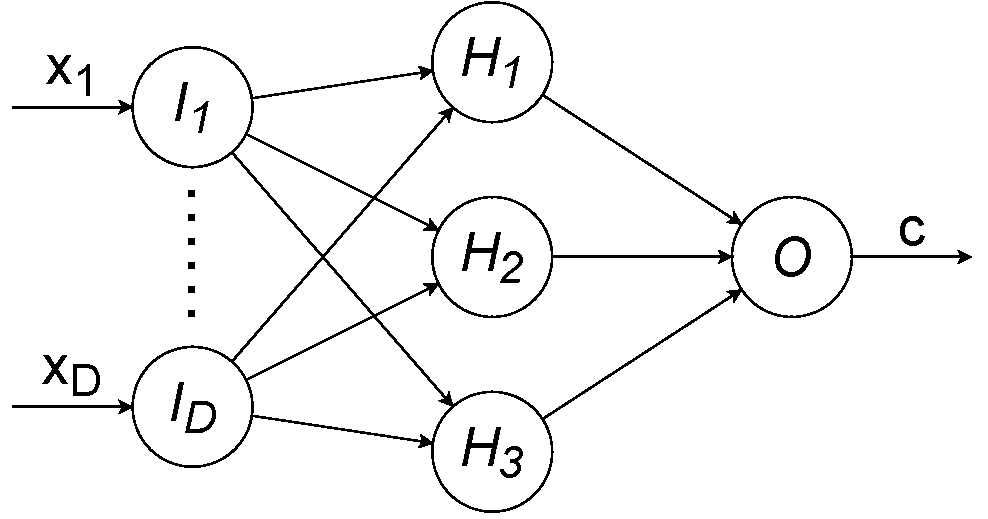
\includegraphics[width=0.5\textwidth]{figuras/estructura_fnn.pdf}
    \caption{Exemple d'estructura d'una xarxa neuronal profunda directa de tres capes: una d'entrada, una oculta i una d'eixida. Cada neurona $n_j$ està connectada amb totes les neurones de la capa posterior $n_{j+1}$.}
    \label{fig:estructura_fnn}
\end{figure}

La funció d'activació, a més d'assignar un valor d'eixida en un rang, apareix per la necessitat d'usar les neurones de forma selectiva, activant les adequades i no actualitzant altres, cosa que permet treballar amb dades no separables linealment.

A continuació es presenten algunes funcions d'activació interessants, així com una petita descripció de cada una:
\begin{itemize}
    \item Sigmoid: es defineix com $f(x)=\frac{1}{1+e^{-x}}$. És senzilla i té un cost temporal baix; el problema més gros és que la derivada genera ràpidament pèrdua d'informació, el que es coneix com a \textit{problema d'esvaïment de gradient}, que no permet a les primeres capes de la xarxa aprendre informació important quan es fa la \textit{retropropagació} (explicada adequadament a continuació).
    \item Tangent hiperbòlica: s'expressa com $f=\frac{e^x-e^{-x}}{e^x+e^{-x}}$, sent el seu rang d'eixida $[-1, 1]$. És típicament preferida sobre la funció Sigmoid, però no resol el problema d'esvaïment de gradient.
    \item ReLu (Rectified Linear Unit): aquesta funció extremadament simple, $f(x)=max(0, x)$, activa les neurones únicament per a valors d'entrada positius. A més, aconsegueix resoldre el problema d'esvaïment de gradient.
    \item Softmax: $f(x)=\frac{e^x}{\sum_i e^{x_i}}$ . Permet interpretar els valors d'eixida de la capa sobre la que s'aplica com una distribució de probabilitat. S'aplica típicament en la capa d'eixida en tasques de classificació.
\end{itemize}

La retropropagació (backpropagation), és l'algorisme que permet aprendre els pesos $w_j$ de l'equació~\ref{eq:prob_neurona} a partir d'un conjunt de dades d'entrenament, d'acord amb algun criteri d'optimització.
En primer lloc, es realitza una inferència cap endavant usant un lot (batch) de dades d'entrenament fins a la capa d'eixida. A continuació, es mesura la divergència entre els valors obtesos a la capa d'eixida i els valors esperats. Aquesta diferència es propaga cap enrere a través de les capes ocultes de la xarxa, modificant apropiadament els pesos de les neurones per minimitzar aquestes diferències. Aquest procés es repeteix de manera iterativa fins convergència. 
Més informació sobre l'algorisme de retropropagació es pot trobar a \cite{rumelhart1986backpropagation}.

Tal i com s'ha mencionat adés, les xarxes neuronals poden tindre més d'una capa oculta. 
Amb aquesta arquitectura, les capes més pròximes a la capa d'entrada aconsegueixen especialitzar-se en xicotets detalls, mentre que les capes més profundes s'especialitzen en característiques més generals i invariants. 
Gràcies a aquest augment de la complexitat i de la grandària d'aquestes xarxes, també ha augmentat la capacitat de processament sobre dades, i és que com s'ha demostrat~\cite{HORNIK1989359}, les DNN compleixen el teorema de l'aproximació universal, que en línies generals diu \guillemotleft Qualsevol funció pot ser \textbf{aproximada} per una xarxa neuronal amb una precisió $p$, tal que  $p < \epsilon$, sent $\epsilon$ un nombre real positiu pròxim a zero, si li proporcionem les suficients neurones\guillemotright. 
En conseqüència, la potència de computació necessària escala de manera proporcional.

\subsection{Xarxes neuronals recurrents}
En tasques com ASR es tracta el processament de seqüències temporals, els components de les quals tenen una gran interdependència interna.
Per exemple, en la producció del llenguatge natural, les seqüències de paraules tenen dependències d'ordre > 1; en la producció fonètica, les seqüències de fonemes també mostren una interdependència (no és el mateix pronunciar una /k/ abans d'una /a/ que d'una /e/, per exemple).
Mitjançant xarxes neuronals recurrents (RNN) és possible aprofitar aquesta informació contextual gràcies a les seues connexions cícliques, i és que les RNNs són, en essència, un tipus de xarxa neuronal amb cicles directes en les seues neurones, que donen lloc a una estructura d'estats interns o memòria~\cite{Yu2015AutomaticSR}.

Una de les arquitectures de xarxes RNN que més rellevància ha generat és la Long Short-Term Memory (LSTM)~\cite{hochreiter1997lstm}, que té com a unitat bàsica la ce\lgem a LSTM, l'encarregada de connectar informació passada a la tasca actual. Aquesta ce\lgem a està formada per tres tipus de portes: la d'entrada, que controla la informació que entra en la ce\lgem a, la de sortida, que controla la informació que ix d'ella i la porta d'oblit, que s'encarrega de recordar o oblidar la informació prèvia de la ce\lgem a. La figura~\ref{fig:estructura_lstm_cell} mostra l'estructura interna bàsica d'una ce\lgem a LSTM.
Per a una explicació més detallada sobre el funcionament d'una xarxa LSTM, es recomana la lectura de~\cite{colah2015lstm}.

\begin{figure}[ht!]
    \centering
    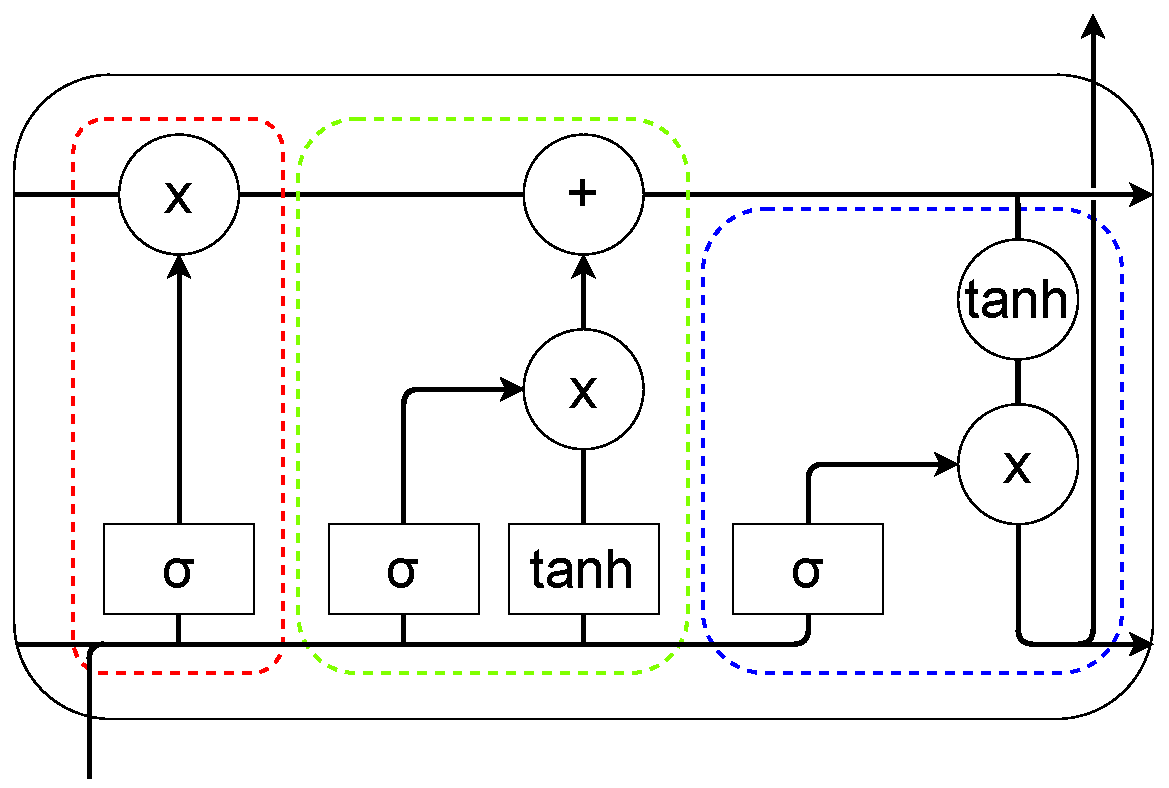
\includegraphics[width=0.8\textwidth]{figuras/estructura_lstm_cell.pdf}
    \caption{Estructura interna d'una ce\lgem a LSTM, on els cercles representen operacions a nivell d'elements, els rectangles representen una capa de xarxa neuronal amb una funció d'activació (sigmoid o $\tanh$). Dues fletxes unint-se representen concatenació de dades, mentre que la seua separació significa que el seu contingut s'envia a diferents localitzacions. L'àrea marcada en roig representa la porta d'oblit, la verda la d'entrada i la blava la de sortida.}
    \label{fig:estructura_lstm_cell}
\end{figure}

Una evolució lògica de les LSTMs son les LSTM bidireccionals (BLSTM), que permeten analitzar les dades en ambdós sentits temporals al mateix temps. Per a aconseguir-ho es duplica l'estructura prèvia, però començant per l'última dada i acabant per la primera. La figura~\ref{fig:lstm_vs_blstm} mostra una comparació visual de la bidireccionalitat aplicada a una xarxa amb la versió unidireccional d'aquesta.

\begin{figure}[ht!]
    \centering
    \begin{subfigure}{0.3\textwidth}
        \centering
        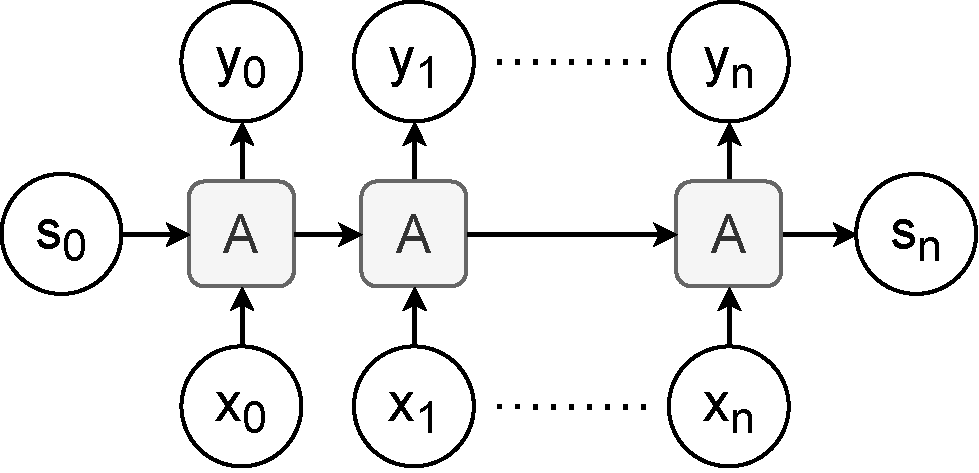
\includegraphics[width=\textwidth]{figuras/lstm_vs_blstm_a.pdf}
        \caption{Xarxa unidireccional}
    \end{subfigure}
    \hfill
    \begin{subfigure}{0.6\textwidth}
        \centering
        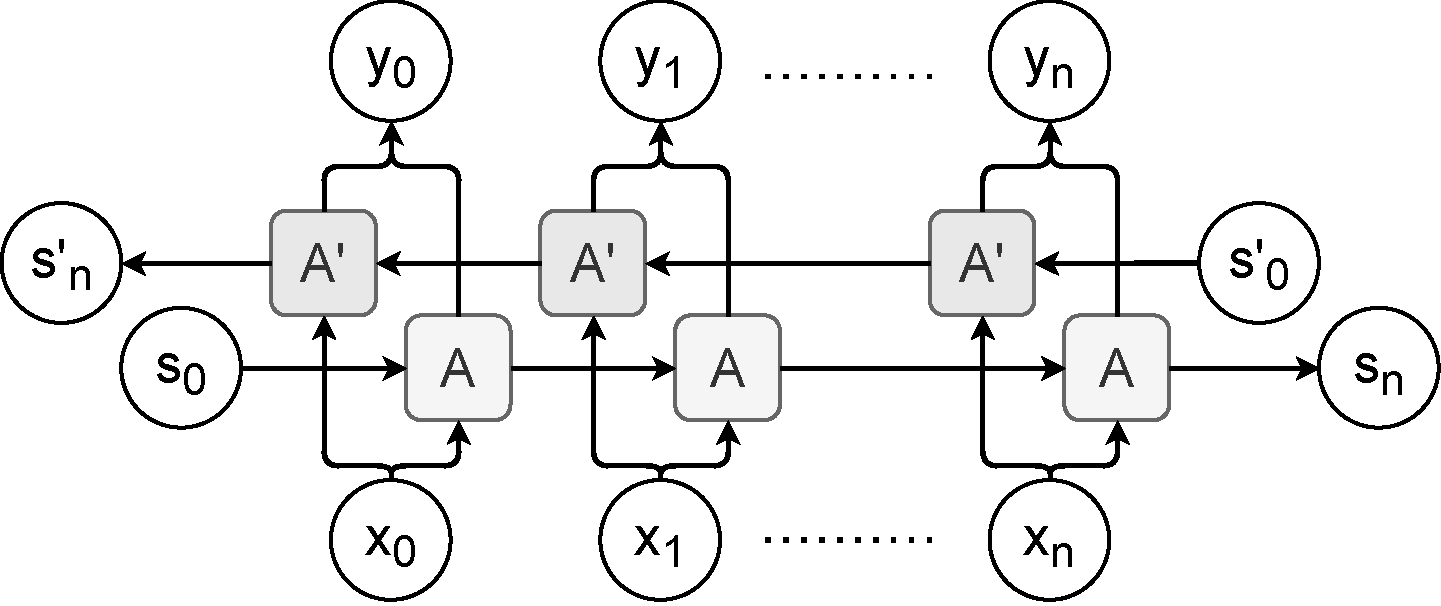
\includegraphics[width=\textwidth]{figuras/lstm_vs_blstm_b.pdf}
        \caption{Xarxa bidireccional}
    \end{subfigure}
    \caption{Comparativa entre una xarxa unidireccional (esquerra) i una altra bidireccional (dreta). A la xarxa bidireccional es pot observar com ambdós estats $s_0$ i $s'_0$ inicien les seues operacions als extrems contraris. Cada subestructura vertical formada pel component d'entrada $x_n$, el d'eixida $y_n$ i la ce\lgem a $A$, o ce\lgem és $A$ i $A'$, és una representació de la xarxa a l'instant $n$.}
    \label{fig:lstm_vs_blstm}
\end{figure}



\subsection{Arquitectura Transformer}

En els últims anys, l'arquitectura Transformer, basada en el concepte d'auto-atenció~\cite{vaswani2017transformers}, s'ha posicionat com l'arquitectura d'avantguarda en múltiples tasques, especialment en el camp del modelat del llenguatge natural.
L'atenció, en aquest camp, és una tècnica que intenta imitar l'atenció cognitiva dels éssers vius, amb l'objectiu focalitzar-se en els conjunts de dades més importants.
Té una estructura encoder-decoder, que assigna seqüències de vectors d'entrada, $(\textbf{x}_1, \dots, \textbf{x}_n)$, a seqüències de vectors d'eixida, $(\textbf{y}_1, \dots, \textbf{y}_n)$, de la mateixa mida. En concret, cada capa està formada per un conjunt de subcapes que contenen xarxes neuronals totalment connectades.
Totes les seves característiques li concedeixen una sèrie d'avantatges front a un RNN: processament en para\lgem el de les dades (en lloc de seqüencial), possibilitat d'atendre potencialment a històries infinites gràcies al mecanisme de d'auto-atenció, entre altres.
Per més informació sobre aquesta arquitectura, remetem a la lectora a~\cite[capítol 9.7]{jurafskySLP}.




\section{Reconeixement automàtic de la parla}
\label{cap02_recon_autom_parla}

ASR és la tecnologia que dota a un sistema automàtic de la capacitat de, partint d'un discurs parlat, obtenir la seqüència de paraules més probable, $\hat{w}$, que la transcriu, mitjançant l'anàlisi de seqüències de vectors de característiques $\textbf{x}$ obtinguts en analitzar el senyal acústic.

Una primera aproximació és l'anomenada sequence-to-sequence, que tracta de modelar directament la probabilitat ``a posteriori'' $P(w | \textbf{x})$. 
El problema d'eixa aproximació és que per entrenar els models sols es poden usar dades de parla etiquetada, i això no és possible en tots els casos per mancança de dades, o bé per l'elevat cost d'etiquetatge d'aquest tipus de dades, especialment si l'etiquetatge és manual. 

L'alternativa són els sistemes híbrids, que opten per aplicar Bayes a la probabilitat a posteriori de la classe (veure Eq.~\ref{eq:form_argmax_classif}). D'aquesta manera, l'Equació~\ref{eq:form_argmax_classif_simpli} es redefineix com segueix:

\begin{equation}\label{eq:form_argmax_classif_ASR}
	\hat{w} = \argmax_{w \in L^{*}} P(w | \textbf{x}) = \argmax_{w \in L^{*}} P(\textbf{x} | w) \, P(w)
\end{equation}
sent $L$ el conjunt de paraules que pot reconèixer el sistema, i $L^{*}$ el conjunt de totes les possibles frases (seqüències de paraules) d'aquest llenguatge. $P(w)$, anomenat model del llenguatge (LM, Language Model), calcula la probabilitat que la frase $w$ forme part del llenguatge $L$, mentre que $P(\textbf{x} | w)$, anomenat model acústic (AM, Acoustic Model), calcula la probabilitat de que aquesta seqüència de paraules $w$ genere la seqüència de vectors acústics $\textbf{x}$.
El gran avantatge de l'aproximació híbrida és que el model del llenguatge es pot entrenar amb una font massiva de dades: text monolingüe en la llengua $L$. Això dona lloc a un component (LM) molt robust, potent i versàtil, i que contribueix de manera decisiva en la millora prestacional dels sistemes ASR. En aquest punt convé ressaltar que aquest treball està centrat en el desenvolupament de models acústics per a sistemes ASR híbrids.

Abans d'entrar en matèria d'algorismes, es contextualitza la dimensió de la problemàtica a resoldre. En primer lloc, la dimensió del vocabulari és clau, ja que influeix directament en la complexitat temporal i espacial del procés d'inferència, reconeixement o decoding, així com en la complexitat del model del llenguatge, que determina el vocabulari del sistema.
Hi ha models que s'entrenen per a reconéixer vocabularis xicotets (p.e. dígits, on hi ha 10 possibilitats) on és més senzill obtenir una gran precisió que en grans models on s'intenta modelar la conversa humana (centenars de milers de paraules).
També cal comentar el domini de les dades a transcriure, no és el mateix transcriure retransmissions esportives que conferències sobre física de partícules (CERN). El vocabulari i les dades d'entrenament poden ser més o menys adaptades a la tasca, i això influeix també en la qualitat del reconeixement.

En segon lloc, el soroll, la reverberació, l'equipament de captura, el nivell de compressió de l'àudio, i altres problemes acústics també dificulten el reconeixement, ja que en un espai amb silenci un micròfon professional s'aconseguirà una mostra de major qualitat que un àudio enregistrat en una revetlla d'estiu amb el telèfon mòbil.
El seu efecte es especialment perjudicial si hi ha una gran diferencia entre les dades de \textit{train} i les d'avaluació: si s'entrena en silenci i bona qualitat, i es reconeix àudio amb reverberació i soroll, la precisió del reconeixement automàtic serà molt baixa.

En tercer lloc, un factor a tindre en compte és el tipus de discurs que es pretén reconéixer: quan una persona parla amb una màquina o llig un text, ho fa sense pressa, intentant vocalitzar i amb una potència regular. 
Per altra banda, el discurs parlat és més complicat de reconéixer a causa de la improvisació, així com el fet que hi ha més d'una interlocutora. Menció apart té la parla so\lgem apada, que es un problema obert avui en dia.

Finalment, una última dimensió a tindre en compte és l'accent de la persona, ja que diferents varietats regionals gasten diferents paraules i possiblement diferents pronunciacions; a més, el discurs parlat d'una xiqueta o d'una persona que està aprenent l'idioma també presenta dificultats si únicament gastem dades de gent adulta durant l'entrenament.

És necessari tindre en compte aquests factors a l'hora de dissenyar una solució, ja que en un sistema de propòsit general la solució passa, evidentment, per emprar la màxima quantitat de dades d'entrenament possibles i, idealment, de fonts i dominis variats. Amb l'objectiu de tindre una mostra de les parlants de la llengua representativa del llenguatge general. Per altra banda, si es desenvolupa un sistema que treballa baix un domini concret, en general s'utilitzaran dades de parla transcrites i de text específiques d'aquest.



\subsection{Modelat acústic}
\label{cap02_asr_am}

El model acústic, $P(\textbf{x}|w)$, és el component de l'aproximació híbrida a l'ASR que s'encarrega de representar probabilísticament la relació entre el senyal acústic i les unitats fonètiques elementals de la pronunciació humana. Aquests, s'entrenen amb dades acústiques de parla transcrita (etiquetada), bé manualment per humans, o bé automàticament amb un sistema ASR pre-existent (self-learning o pseudo-labeling).

Formalment, podem definir un model ocult de Markov $M$ de la següent manera:

\begin{equation}
M=(Q, \Sigma, \pi, A, B)
\end{equation}
on $Q$ és un conjunt finit d'estats, $\Sigma$ és un conjunt finit de símbols que es poden emitir (també nomenat alfabet), $\pi$ és un vector de probabilitats inicials, $A$ és una matriu de probabilitats de transició, que guarda la probabilitat de transitar d'un estat $q$ a qualsevol altre estat $q'$, i $B$ és una matriu de probabilitats d'emissió, que guarda les probabilitats d'emitir un símbol $x_t$ en un estat $q_t$ a l'instant de temps $t$.

Els models acústics dels sistemes ASR híbrids treballen sobre un nombre indefinit de finestres temporals, per aquesta raó es basen en models ocults de Markov (HMMs, Hidden Markov Models). Un HMM és un model probabilístic que serveix per modelar processos Markovians, és a dir, processos aleatoris dependents del temps, com és el cas particular de la fonologia humana. Concretament, els HMMs s'usen per modelar fonemes i inclús trifonemes (fonemes amb context).

Els HMM es basen en les dues assumpcions de Markov:
\begin{itemize}
    \item La probabilitat que, en un instant $t$, el model es trobe en un estat $q_t$, solament depén de l'estat $q_{t-1}$, a l'instant immediatament anterior. A més, les probabilitats de transicionar d'un estat a un altre son estacionàries en el temps, és a dir, són independents d'en què instant $t$ es donen.
    \item La probabilitat d'emissió d'una observació $x_t$ depen únicament de l'estat en el qual es produeix l'observació, $q_t$, i no de cap altra observació o emissió anterior. Açò és:

    \begin{equation}
        P(x_i|q_1, \dots, q_i, \dots, q_T, x_1, \dots, x_i, \dots, x_T) = P(x_i|q_i)
    \end{equation}
\end{itemize}

La figura~\ref{fig:estructura_hmm} mostra l'estructura general del HMM explicat.

\begin{figure}[ht!]
\centering
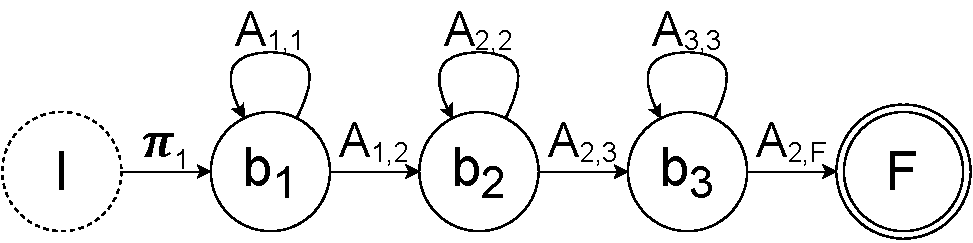
\includegraphics[width=0.55\textwidth]{figuras/estructura_hmm.pdf}
\caption{Representació d'un HMM. Podem apreciar els tres estats $b_1$, $b_2$ i $b_3$ que representen l'inici, la part central i el final del fonema. També s'observen els estats Inicial i Final, que indiquen quan ha començat i acabat el reconeixement del fonema en qüestió.}
\label{fig:estructura_hmm}
\end{figure}

Per tant, la probabilitat que el model HMM associat a un fonema $f$ genere o explique la seqüència acústica $\textbf{x}$ és:

\begin{equation}
    P_f(\textbf{x}) = \sum_{q \in Q} \prod_{t=1}^{|q|} P(q_t|q_{t-1}) P(\textbf{x}_t|q_t)
    \label{eq:hmm_prob}
\end{equation}
on $q_t$ és el $t$-èsim estat assolit per la seqüència d'estats $q$, $\textbf{x}_t$ és $t$-èsim vector de la seqüència de vectors $\textbf{x}$, $P(q_t|q_{t-1})$ és la probabilitat de transitar d'un estat $q_{t-1}$ a un estat $q_t$, i $P(\textbf{x}_t|q_t)$ és la probabilitat d'emissió del vector $\textbf{x}_t$ a l'estat $q_t$.

Pel que fa a les probabilitats d'emissió, $P(\textbf{x}_t|q_t)$, tradicionalment s'han modelat mitjançant mixtures de Gaussianes (GMMs)~\ref{cap02_mixtures}, entrenades amb l'algorisme Expectation-Maximization (EM). En aquest cas, parlem de models acústics basats en GMM-HMMs.

Aquests models acústics, quan són acoblats juntament amb el model del llenguatge a un sistema ASR, ajunten els estats Inicial i Final de fonemes ($P_f(\textbf{x})$ o, equivalentment, $P(\textbf{x}|f)$) o trifonemes consecutius. Ho fan d'acord amb la informació proporcionada per diccionaris de pronunciació fonètics (model lèxic), per a conformar HMMs a nivell de paraula: $P_w(\textbf{x})$, o directament, $P(\textbf{x}|w)$, el model acústic pròpiament dit. 

Més recentment, en l'última dècada, les xarxes neuronals, gràcies al seu gran poder discriminatiu, han reemplaçat els GMMs en el modelat de les probabilitat d'emissió. 
Açò va permetre generar models més robusts, ja que no fan cap assumpció sobre l'origen de les dades, que també permeten obtenir uns resultats significativament millors\cite{hinton2012}. 
Per tal de poder explotar el potencial de les DNNs en l'estimació de les probabilitats d'emissió, $P(\textbf{x}_t|q_t)$, primer s'aplica el teorema de Bayes sobre l'equació~\ref{eq:hmm_prob}:

\begin{equation}
P_f(\textbf{x}) = \sum_{q \in Q} \prod_{t=1}^{|q|} P(q_t|q_{t-1}) \frac{P(\textbf{x}_t) P(q_t|\textbf{x}_t)}{P(q_t)} 
\end{equation}

A continuació, considerant l'equivalència formal dels HMMs a nivell de fonema $P_f(\textbf{x})$, amb els HMMs a nivell de paraula $P_w(\textbf{x})$ o $P(\textbf{x}|w)$, així com que, en la cerca, s'aplica l'aproximació de Viterbi per obtenir el camí $q$ més probable, podem reescriure l'equació~\ref{eq:form_argmax_classif_ASR} com segueix:

\begin{equation}
	\hat{w} = \argmax_{w \in L^{*}} P(w | \textbf{x}) = \argmax_{w \in L^{*}} \max_{q \in Q} \prod_{t=1}^{|q|} P(q_t|q_{t-1}) \frac{P(\textbf{x}_t) P(q_t|\textbf{x}_t)}{P(q_t)} \, P(w)
    \label{eq:cerca_nivell_paraules}
\end{equation}

A l'igual que en el pas de l'equació~\ref{eq:form_argmax_classif} a l'equació~\ref{eq:form_argmax_classif_simpli}, tenim que $P(\textbf{x}_t)$ és constant i independent de la classe de l'objecte, raó per la qual podem obviar-la i estalviar-nos calcular-la. Pel que fa a $P(q_t)$, les probabilitats a priori dels estats HMM, poden calcular-se mitjançant l'aprenentatge amb dades d'entrenament i normalitzant els comptes de cada estat $q_t$ durant aquest entrenament.
%Alguns dels actuals sistemes estat de la tècnica gasten dues aproximacions per a estimar $P(q_t|x_t)$, i conseqüentment, les probabilitats d'emissió:
Per últim, $P(q_t|\textbf{x}_t)$, i conseqüentment, les probabilitats d'emissió del HMM integrat, poden ser modelades per xarxes neuronals de tipus FF-DNN (models FF-DNN-HMM)~\cite{hinton2012}, Convolucionals (models CNN-HMM)~\cite{6857341}, BLSTM (models BLSTM-HMM)~\cite{mllp2020} o Transformer (models T-HMM)~\cite{wang2020transformers_asr}.

Aquest treball se centra en el desenvolupament d'un sistema ASR híbrid BLSTM-HMM, tecnologia que encara demostra estar a la avantguarda de la tècnica~\cite{jorge2021iberspeech}.
La lectora pot trobar més informació sobre els models ocults de Markov a l'àmbit del ASR a \cite[capítol 8.4]{jurafskySLP}.



\subsection{Preprocés i extracció de característiques}
\label{cap02_preprocessat_acustic}
El primer pas que cal donar per a construir models acústics és el preprocès i l'extracció de característiques de les dades d'entrenament per tal d'obtenir els vectors de característiques $\textbf{x}$. 

En primer lloc, cal obtenir la versió digital de l'ona acústica. Aquesta conversió es divideix en dues tasques: d'una banda, cal realitzar un mostreig, consistent en mesurar l'amplitud de l'ona en un instant particular de temps.
Seran necessàries un mínim de dues mostres per cada cicle de l'ona (una per a la part positiva de l'ona i l'altra per a la negativa). A major quantitat de mostres, major qualitat, però tenint en compte que la màxima freqüència que podem mesurar és la meitat de la freqüència de mostreig (freqüència de Nyquist\cite{grenander1959probability}).
Per a l'ASR és suficient amb mostres de 16 KHz, ja que els principals sons de la fonologia humana es troben baix de l'espectre dels 8 KHz.
Per altra banda, cal quantificar la informació, codificant el valor de cada amplitud mesurada, típicament, en nombres enters de 16 bits.

A continuació es generen una sèrie de finestres temporals de les quals s'extrauen els vectors de característiques. En aquestes finestres cal fixar tres paràmetres: la mida de la finestra (en ms), el retard entre una finestra i la seua adjacent (en ms), i la forma de la finestra.
La figura~\ref{fig:finestres_temporals} representa el procés de generar diverses finestres per a poder extraure vectors de característiques.
\begin{figure}[ht!]
    \centering
    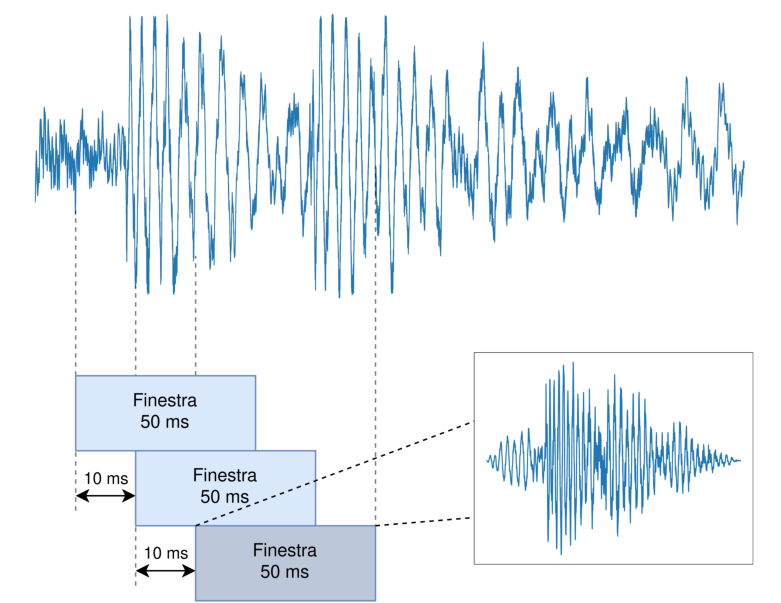
\includegraphics{figuras/finestres_temporals.pdf}
    \caption{Finestres amb forma de Hamming de 50 ms amb un retard de 10 ms.}
    \label{fig:finestres_temporals}
\end{figure}
Típicament, s'usen finestres de Hamming, ja que la finestra rectangular talla l'àudio de forma abrupta. Açò és resol atenuant ambdós costats de la finestra segons la fórmula:

        \begin{align}
            w(n)_{Rectangular} &=
                \begin{dcases}
                    1 & 0 \leq n \leq L-1 \\
                    0 & \text{altre cas}
                \end{dcases} \\
            w(n)_{Hamming} &=
                \begin{dcases}
                    0.54 - 0.46 \cos \frac{2 \pi n}{L} & 0 \leq n \leq L-1 \\
                    0 & \text{altre cas}
                \end{dcases}
        \end{align}
        A la figura~\ref{fig:comparativa_finestres} s'aprecia la diferència d'ambdues formes.

        \begin{figure}[!ht]
             \centering
             \begin{subfigure}{0.4\textwidth}
                 \centering
                 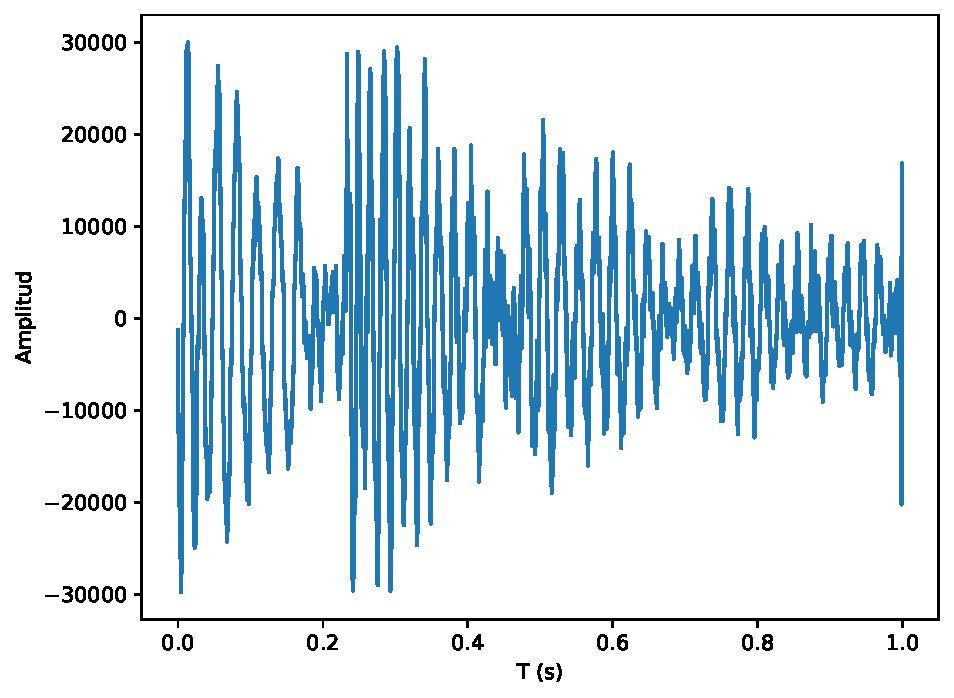
\includegraphics[width=\textwidth]{figuras/finestra_rect.pdf}
                 \caption{Finestra rectangular}
             \end{subfigure}
             \begin{subfigure}{0.4\textwidth}
                 \centering
                 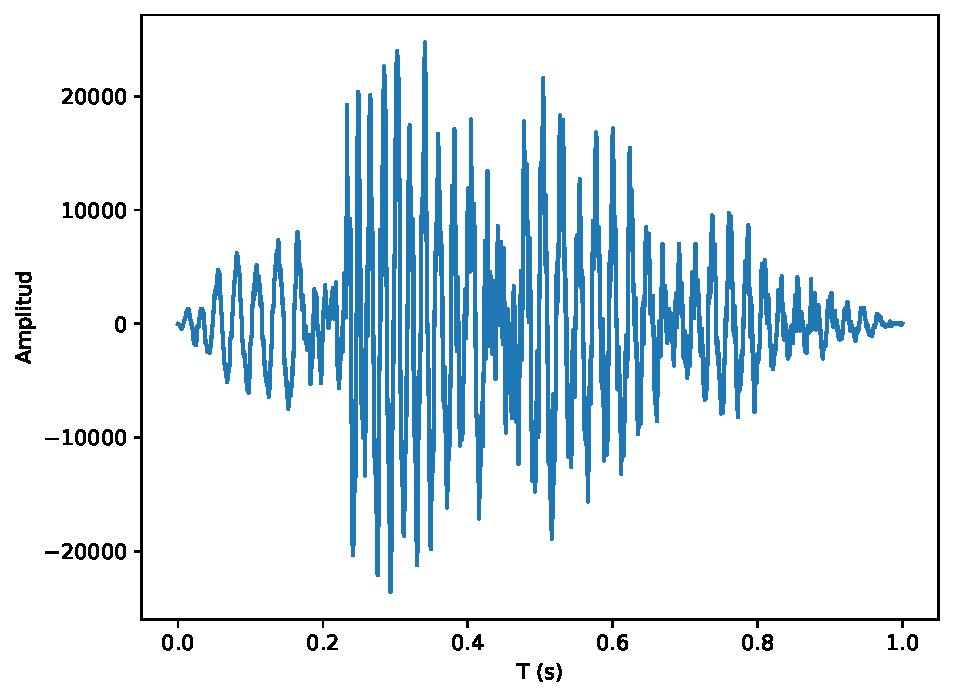
\includegraphics[width=\textwidth]{figuras/finestra_hamm.pdf}
                 \caption{Finestra de Hamming}
             \end{subfigure}
             \caption{Comparativa de la mateixa mostra acústica baix les dues formes de finestra. S'observa l'atenuament en els extrems de la finestra de Hamming.}
             \label{fig:comparativa_finestres}
        \end{figure}



El següent pas és extraure la informació de cada finestra. Es realitza una transformada discreta de Fourier (Discrete Fourier Transform, DFT), que extrau l'energia del senyal en diferents bandes de freqüència. Aquesta transformada es defineix com:

    \begin{equation}
        X_k = \sum_{n=0}^{N-1} x_n \cdot e^{- \frac{2 \pi i}{N} kn} \quad  \forall k \in{0, \dots, N-1},
    \end{equation}
    on $i$ és la unitat imaginaria i $e^{- \frac{2 \pi i}{N}}$ és l'N-ésima arrel de la unitat.

Típicament, s'usa l'algorisme de \textit{transformada ràpida de Fourier} (\textit{FFT, Fast Fourier Transform}) per a calcular la \textit{DFT}. Aquesta implementació es molt eficient, però solament funciona per a valors de $N$ que siguen potències de 2.
    Per a més informació sobre la transformada discreta de Fourier, es recomana a la lectora~\cite{mathews2012complex}.

En quart lloc, degut a que l'oïda humana no percep de la mateixa manera totes les bandes, és molt més sensible a freqüències baixes que a altes, cal modelar aquesta percepció per millora notablement la qualitat del reconeixement de la parla. S'assoleix mitjançant un banc de filtres Mel~\cite{8732232}.
El nombre de dimensions del vector resultant és igual al nombre de filtres que formen el banc. La figura~\ref{fig:mel_filterbank} exemplifica un banc de filtres triangulars que implementen aquesta idea.

    \begin{figure}[ht!]
        \centering
        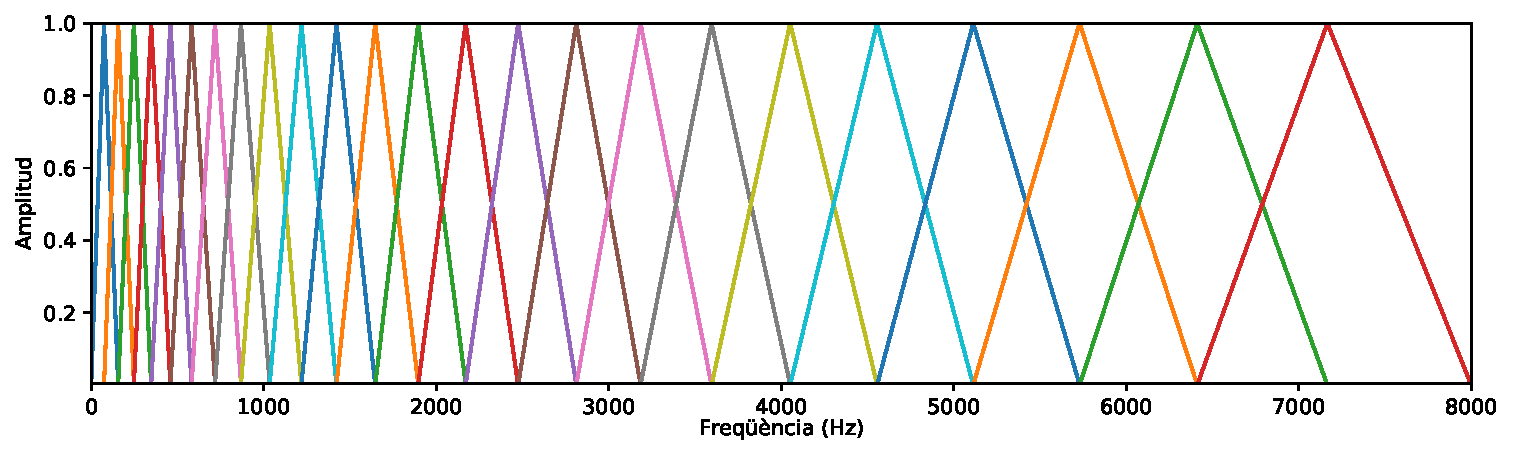
\includegraphics[width=\textwidth]{figuras/mel_filterbank.pdf}
        \caption{Banc de filtres Mel. Cada filtre triangular està espaiat logarítmicament mitjançant l'escala mel.}
        \label{fig:mel_filterbank}
    \end{figure}
A l'eixida d'aquest pas, tenim els vectors de característiques Filterbanks. 
A continuació s'aplica l'algorisme de \textit{transformada cosinus discreta} (\textit{DCT, Discrete Cosine Transform}) i, finalment, es normalitzen les mostres amb l'objectiu de minimitzar les seues diferències. D'aquesta manera xicotetes diferències en la pronunciació i la sonoritat perden rellevància, augmentant la capacitat de generalització del model.
L'eixida d'aquest preprocès són els vectors de característiques MFCC (Mel Frequency Cepstral Coefficient), un per cada frame.



\subsection{Modelat del llenguatge}
\label{cap02_asr_lm}

El model del llenguatge és l'altre component principal del sistema híbrid que representa l'estructura pròpia del llenguatge modelant $P(w)$. En altres paraules, calcula la probabilitat que una paraula $w_i$ aparega donada una història o context previ $w_1, w_2, \dots, w_{i-1}$.
El fet que els models del llenguatge s'entrenen amb dades de text monolingüe (molt abundants i de fàcil accés), ens permet entrenar models robusts i potents. De fet, aquest és el principal motiu que ens fa optar per una aproximació híbrida i que assoleix que ara mateix siga l'aproximació més puntera enfront dels sistemes end-to-end.

Existeixen diferents aproximacions al modelat de llenguatge. Tradicionalment, s'ha emprat l'aproximació estadística basada en comptes, representada pels models de n-grames: seqüències contigues d'$n$ paraules a les quals se solen referir pel nombre d'aquestes (unigrama, bigrama, trigrama, etc.). El model del llenguatge utilitzat al sistema final empra n-grames per a aproximar $P(w)$ com la probabilitat d'una paraula $w_i$ donada una història $h_i=w_1 w_2 \dots w_{i-1}$ (seqüència prèvia de paraules). Pot expressar-se mitjançant la probabilitat condicional com $P(w_i|h_i)$, o formalment:

\begin{equation}
P(w) \approx \prod_{i=1}^{I+1} P(w_i|w_{\max(i - n + 1, \ 0)}^{i-1})
\end{equation}
on I es la grandària de $w$, $n$ la mida de l'n-grama, $w_i^{i+j}$ representa la seqüència de paraules $(w_i, w_{i+1}, \dots, w_j) \in w$, i $w_0$ i $w_{I+1}$, sengles estats especials que representen els \textit{tokens} especials d'inici i final de frase. D'aquesta manera, un n-grama de segon ordre o bigrama, permet contextualitzar únicament la paraula anterior a l'actual i un trigrama les dues anteriors. Per exemple, en la frase \guillemotleft Llança el dau de vint cares\guillemotright, la probabilitat que la paraula \guillemotleft cares\guillemotright ~aparega després de la paraula \guillemotleft vint\guillemotright ~pot expressar-se amb un model trigrama com:

\begin{align}
    P( \text{ \guillemotleft de vint cares\guillemotright } ) = 
    &P( \text{ \guillemotleft de\guillemotright } | \text{ IDF } ) \nonumber \\
    &P( 
        \text{ \guillemotleft vint\guillemotright } | 
        \text{ IDF}, \text{ \guillemotleft de\guillemotright } 
    )  \\
    &P(
        \text{ \guillemotleft cares\guillemotright } | 
        \text{ \guillemotleft de vint\guillemotright }
    )  \nonumber \\
    &P(
        \text{ FDF } | 
        \text{ \guillemotleft vint cares\guillemotright }
    ) \nonumber
\end{align}
on $IDF$ i $FDF$ són els tokens especials de \guillemotleft Inici de frase\guillemotright ~i \guillemotleft Final de frase\guillemotright. 

Més recentment, els models de llenguatge continus o neuronals, s'han imposat clarament als models de n-grames, especialment els basats en mecanismes d'autoatenció~\cite{wang2019transformers_lm, baqueroarnal20_interspeech}, com l'arquitectura Transformer, exhibint una capacitat d'atenció potencialment infinita a qualsevol paraula de la història prèvia, en clar contrast amb les severes limitacions dels n-grames, que sols retenen una història de $n-1$ paraules, i on típicament $n \leq 4$.
%L'aplicació de l'arquitectura transformer al model del llenguatge ha assolit millors resultats que els anteriors models estats de la tècnica~\cite{wang2019transformers_lm}~\cite{baqueroarnal20_interspeech}.

En aquest treball s'utilitzaran models de llenguatge de n-grames i Transformer proporcionats per investigadors del grup de recerca MLLP, per aquesta raó, el seu entrenament i la seua optimització queda fora de l'abast d'aquest treball.

\subsection{Descodificació / Reconeixement}
\label{cap02_asr_decoder}

La descodificació és l'etapa en la qual ambdós models, l'acústic i el del llenguatge, es combinen per a trobar la seqüència de paraules més probable per a la mostra acústica donada d'acord amb l'equació~\ref{eq:cerca_nivell_paraules}. Per a fer-ho es genera un multigraf dirigit amb totes les paraules del vocabulari, sent cada node, un fonema de la paraula. Una simplificació d'aquesta estructura pot observar-se a la Figura~\ref{fig:decoder_simpli}.

\begin{figure}[ht!]
\centering
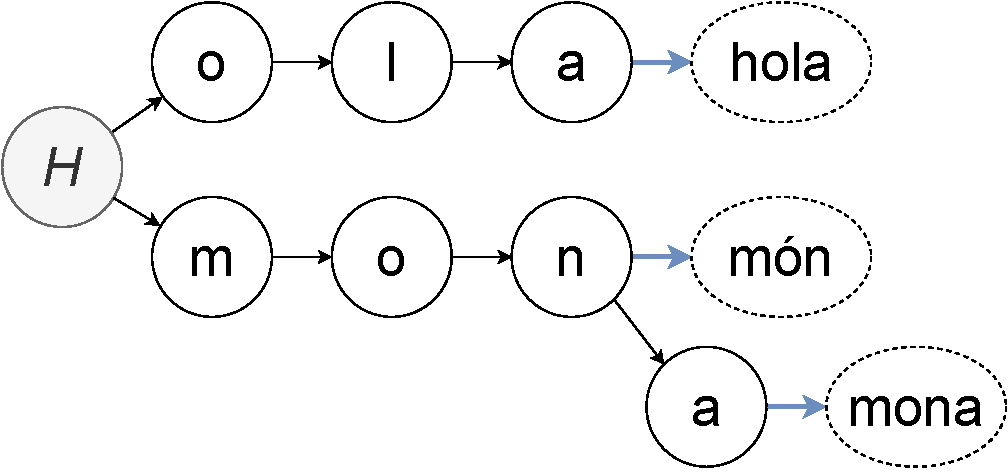
\includegraphics[width=0.5\textwidth]{figuras/espai_cerca.pdf}
\caption{Exemple d'un graf de cerca capaç de reconéixer una paraula. Per motius de brevetat es considera un vocabulari de solament tres paraules: \guillemotleft hola\guillemotright, \guillemotleft món\guillemotright i \guillemotleft mona\guillemotright. L'estat inicial, $H$, denota la història actual. En concret, les fletxes blaves indiquen l'instant exacte en el qual està calculada la probabilitat d'una paraula, que comporta realitzar una consulta explícita al model de llenguatge, per exemple \guillemotleft hola\guillemotright, donada la història, $P(paraula | H)$.}
\label{fig:decoder_simpli}
\end{figure}

S'ha de tindre en compte que l'espai de cerca és, en qualsevol cas, molt gran, ja que totes les paraules del vocabulari del sistema són assolibles des de qualsevol història. A més, durant la descodificació, aquestes decisions es prenen a escala de frame. Aquest mecanisme posa en compromís la latència del sistema i pot no servir per a tasques d'ASR en temps real.

Una solució parcial és aplicar tècniques de poda de l'espai de cerca, de tipus beam-search, que solament mantinguen un subgrup d'hipòtesis més probables en cada instant. Però presenta un altre inconvenient: una hipòtesi descartada pot ser realment més encertada que una que es mantén, ja que durant la cerca, solament es té en compte l'opinió del model acústic, mentre que el model de llenguatge sols aporta el seu coneixement quan el procés de descodificació transita d'un estat fonema a un estat paraula.
Per solucionar-ho, s'usen taules estàtiques de look-ahead~\cite{jorge19_interspeech}, un algorisme recursiu que, des de les fulles de la cerca (totes les paraules del vocabulari), va assignant a cada estat la màxima probabilitat assolible des d'ell, segons el model del llenguatge. D'aquesta manera, durant la cerca, quan hi ha una bifurcació solament cal restar a l'estat actual la probabilitat actual màxima del LM i sumar la màxima assolible per cada camí. 
D'aquesta manera, durant la cerca, totes les hipòtesis tenen també informació aportada pel model del llenguatge i la quantitat de consultes que se li realitzen es redueix dràsticament.

\subsection{Avaluació de sistemes ASR}
\label{cap02_asr_avaluacio}

Els sistemes ASR s'avaluen de forma objectiva mitjançant la taxa d'error per paraula (WER, Word Error Rate), que es defineix com la mínima distància entre les transcripcions obtingudes pel sistema i les originals, utilitzant les dades de \textit{development} i \textit{test}.
Aquesta mètrica és similar a la distància de Levenshtein: permet insercions, substitucions i eliminacions a escala de paraula. Es defineix com:

\begin{equation}
WER = \frac{I + S + E}{R}\cdot 100
\end{equation}
on $I$, $S$ i $E$ són, respectivament, el nombre d'insercions, substitucions i eliminacions necessàries perquè la nostra transcripció siga idèntica a l'original, i $R$ és el total de paraules de la transcripció.
El WER pot entendres, de forma intuïtiva, com el percentatge de paraules de la transcripció automàtica que cal esmentar per a obtenir la transcripció correcta de referència.

No obstant això, els components principals dels sistemes ASR, això és, el model acústic i el model del llenguatge, estan desenvolupats i optimitzats de forma independent i amb diferents fonts de dades. Per tant, durant l'etapa de desenvolupament del sistema ASR, el seu rendiment individual es mesura utilitzant altres mètriques. 
En el cas dels models acústics basats en xarxes neuronals, aquests estan entrenats minimitzant la taxa d'error de classificació de frames (FER, Frame Error Rate) en un conjunt de desenvolupament donat.
FER està definida com el nombre de frames incorrectament classificats dividit entre el total de frames analitzats:

\begin{equation}
FER = \frac{F_{\text{incorrectes}}}{F_{\text{totals}}}
\end{equation}



    % ---------------------------------------------------------------------
    % ---------------------------------------------------------------------
    % ---------------------------------------------------------------------

    \chapter{Entrenament de models acústics}
    \label{cap03__}

    % ---------------------------------------------------------------------
    % ---------------------------------------------------------------------
    % ---------------------------------------------------------------------

    % Procediment (recepta explicada)
    %
En el present capítol es descriu el procediment i les tècniques emprades per l'entrenament de models acústics híbrids de tipus BLSTM-HMM.
Inicialment, la Secció~\ref{cap03_intro} resumeix el procés seguit per generar un model acústic.
A continuació, la Secció~\ref{cap03_prepro} explica els passos necessaris per preparar les dades que s'empraran durant els entrenaments dels diferents models.
En tercer lloc, la Secció~\ref{cap03_gmmhmm} descriu el procediment que cal seguir per entrenar un model GMM-HMM.
La Secció~\ref{cap03_dnnhmm} explica com entrenar un model FF-DNN-HMM.
Finalment, la Secció~\ref{cap03_blstmhmm} detalla com entrenar un model BLSTM-HMM.
 
\section{Introducció}
\label{cap03_intro}

El procediment d'entrenament de models híbrids està dividit principalment en tres fases.
La Figura~\ref{fig:resum_am} mostra, de manera esquemàtica, aquestes fases.
Primerament, s'entrena un model acústic de tipus GMM-HMM, consistent en un model ocult de Markov inicial, en el que les probabilitats d'emissió dels estats es modelen amb una mixtura de Gaussianes. Aquest model s'usa a continuació per a inicialitzar i entrenar un model híbrid FF-DNN-HMM. De la mateixa manera, aquest segon model es fa servir per a inicialitzar el tercer i últim model BLSTM-HMM.

L'aproximació d'entrenar models auxiliars ve motivada pel fet que la BLSTM no pot entrenar-se directament. 
Per poder modelar $P(q_t|\textbf{x}_t)$ amb una BLSTM, necessitem obtindre les etiquetes $q_t$ associades a cada vector acústic d'entrada $\textbf{x}_t$, és a dir, necessitem els alineaments més probables $(q_t, \textbf{x}_t), \; \in {1,T}$.
Açò s'obté inicialment amb el model auxiliar GMM-HMM, ja que permet modelar directament $P(\textbf{x}_t|q _t)$ sense cap prerequisit previ amb un model generatiu com són les mixtures de Gaussianes.
Amb les dades alineades d'aquest model, és a dir, amb els diferents vectors de característiques emparellats als senones que representen, podem entrenar una xarxa neuronal, en aquest cas una FF-DNN. 
La raó per entrenar una FF-DNN i no passar directament a una BLSTM és perquè les FF-DNN donen alineaments més precisos, de millor qualitat, per entrenar el model final BLSTM-HMM, gràcies a la seua capacitat discriminativa i la seua robustesa front a soroll i possibles \textit{outlayers}, és a dir, frames incorrectament alineats pel model GMM-HMM.
%En el cas que tinguérem ja un model entrenat i amb les dades alineades, podríem botar-nos aquesta part de la tasca. De fet, aquest mateix sistema podrà ser reentrenat amb dades noves mitjançant l'alineament de les seues dades en un futur si fora necessari.

    \begin{figure}[h]
        \centering
        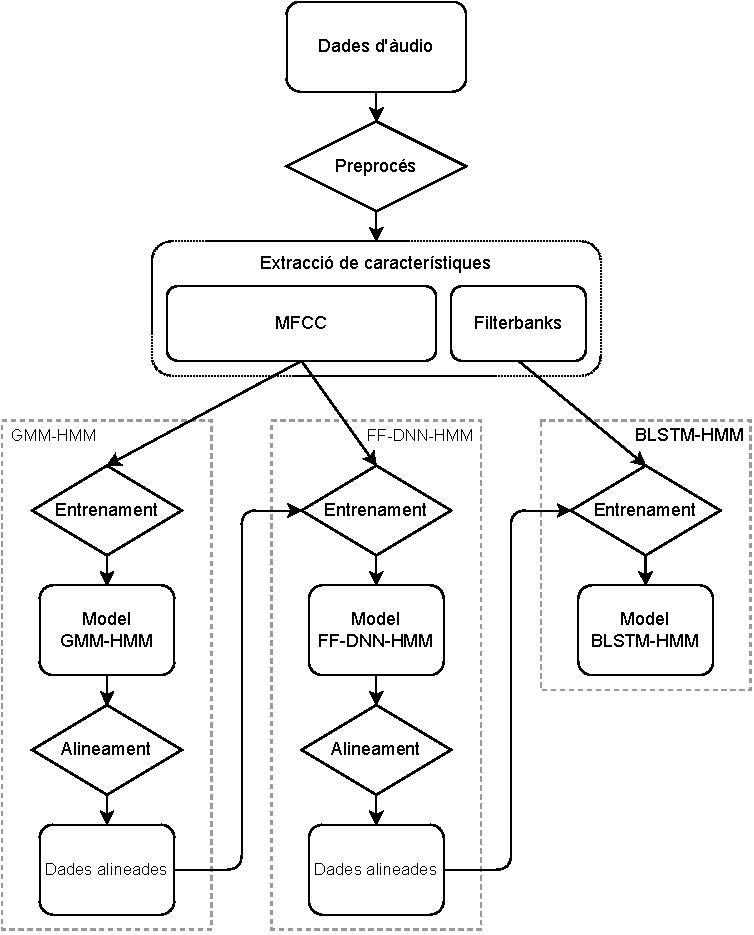
\includegraphics{figuras/resum_am.pdf}
        \caption{Diagrama que mostra els diferents passos seguits per a la creació del model acústic.}
        \label{fig:resum_am}
    \end{figure}

\section{Preprocés i extracció de característiques}
\label{cap03_prepro}

En primer lloc, quant al preprocés, s'apliquen una sèrie de transformacions sobre el text de les transcripcions de la parla per eliminar informació que no afecta a la pronunciació, ja que encara que siguen correctes, aquestes presenten una varietat d'informació que és irrellevant per a obtenir la correcta pronunciació de les mostres: majúscules, signes de puntuació o dígits.
A continuació, es genera una transformació de paraules a seqüència de fonemes, usant un diccionari de pronunciació o model lèxic, generat de forma manual amb coneixement expert, o de forma automàtica mitjançant models estadístics~\cite{BISANI2008434}.

En segon lloc, pel que respecta al pas d'extracció de característiques, s'aplica el procés descrit a la Secció~\ref{cap02_preprocessat_acustic} per a extreure vectors de característiques de tipus MFCC per a l'entrenament dels models GMM-HMM i FF-DNN-HMM, i de tipus Filterbank per a l'entrenament del model final BLSTM-HMM. 


\section{Entrenament de GMM-HMM}
\label{cap03_gmmhmm}

Les raons per entrenar un model GMM-HMM són, per una banda, obtenir una topologia de senones, és a dir, definir el conjunt de classes del model acústic; i per altra banda, aconseguir un alineament de les dades d'entrenament per poder entrenar un model acústic neuronal de majors prestacions en passos posteriors.
    
Aquest procés requereix un conjunt de mostres d'entrenament dels vectors de característiques MFCC, junt a les seues transcripcions fonètiques.
Per entrenar els HMMs, usarem l'algorisme d'expectativa-maximització Baum-Welch, algorisme iteratiu que optimitza els paràmetres d'un model amb variables ocultes. És a dir, es tracta de descobrir els camins $q$ que millor expliquen les seqüències d'observacions $x$ d'entrenament.
Les taules de transicions seran reutilitzades pels diferents models especificats ací.

Primer s'entrenen HMMs de monofonemes amb Gaussianes diagonals, inicialitzades amb l'estimació d'una única Gaussiana global amb la mitjana i la variància dels frames d'entrenament.
En aquest cas, cada HMM modela un únic monofonema, però per necessitat d'identificar el context immediat s'introdueixen els trifonemes. Un trifonema, com el seu nom indica, és un conjunt de tres fonemes: el central, que dona la informació principal i és vertader fonema a identificar, i els laterals, que afegeixen el context necessari per a una millor classificació del fonema central. D'aquesta manera, un trifonema sol definir-se com $S_1-S_2+S_3$, on $S_2$ és el fonema central, a ser identificat, i ambdós $S_1$ i $S_3$ el seu context esquerre i dret, respectivament.

A continuació, s'entrenen HMMs de trifonemes amb Gaussianes diagonals, sent inicialitzats amb els paràmetres del monofonema central del model anterior.
No obstant, els models HMMs de trifonemes presenten un problema important. Posem d'exemple el Francés, una llengua amb 35 fonemes. Aquests generen potencialment 42875 trifonemes diferents, cadascun amb tres estats. Això implica un total de 128625 estats, tots i cadascun d'ells equipats amb una Gaussiana o mixtura de Gaussianes. A més, durant l'entrenament hi haurà trifonemes que apareixeran poques vegades o que directament no existeixen en el corpus de train.
Aquests problemes es solucionen mitjançant l'algorisme CART, que ens permet detectar i agrupar estats de HMMs de diferents trifonemes amb poca o nu\lgem a observació estadística que son similars des d'un punt de vista estadístic. Així, estats agrupats s'uneixen per conformar un únic estat nugat (\textit{tied-state}) compartit per múltiples models de HMMs de trifonemes lligats.
%Algunes de les preguntes que es realitzen durant la creació d'aquest arbre són \guillemotleft està a la dreta/esquerra hi ha una vocal?\guillemotright o \guillemotleft està a principi de paraula?\guillemotright.
%L'arbre CART es crea de forma automàtica mitjançant un script amb un set de regles que fa totes les preguntes bàsiques possibles a ambdós costats (dreta i esquerra) i una sèrie de preguntes extra per a casos particulars de la llengua. 
Per a una explicació més detallada del CART, així com de possibles tècniques per optimitzar-lo, es recomana a la lectora dirigir-se a \cite[cap. 18.1]{pml1Book}.

Una vegada generat el conjunt d'estats nugat, s'inicialitza el model de trifonemes nugats amb Gaussianes diagonals, on cada Gaussiana obté el valor inicial de la Gaussiana que representa la seua fulla de l'arbre CART, emprant les mateixes taules de transicions. Aquest model s'entrena amb diverses iteracions de l'algorisme de EM.

Finalment, s'entrena el model GMM-HMM de trifonemes lligats, amb Mixtures de Gaussianes diagonals. Aquest és un procés iteratiu i molt costós, doncs cada model utilitza l'anterior per a entrenar-se. S'entrenen diferents models, cadascun amb una mixtura de $2^i : 0 \le i \le N$ components per cada estat nugat del model, on $N$ es un paràmetre a fixar.

Com s'ha introduït a l'inici del capítol, és necessari obtenir alineaments dels frames d'entrenament a nivell d'estat de model HMM per poder entrenar el model FF-DNN-HMM. 
Per aconseguir-ho, s'usa el model GMM-HMM definitiu de trifonemes lligats amb mixtures de Gaussianes, el qual calcula la seqüència d'estats $\hat{q}$ del model de Markov que millor explica cadascuna de les mostres $\textbf{x}$ d'entrenament. Convé destacar que la seqüència d'estats $\hat{q}$ revel·la la seqüència de trifonemes que, d'acord amb el model acústic, millor descriu l'observació acústica $\textbf{x}$.

    
\section{Entrenament de FF-DNN-HMMs}
\label{cap03_dnnhmm}

En aquest pas, es reutilitza la topologia (conjunt d'estats i probabilitats de transició) del model GMM-HMM. Sols s'entrena la FF-DNN encarregada de modelar $P(q_t|\textbf{x}_t)$, tal i com s'ha detallat en la Secció~\ref{cap02_asr_am}

La FF-DNN té en l'eixida una capa softmax amb tantes neurones com senones té el model acústic. Aquesta s'entrena diverses èpoques amb els alineaments de la GMM-HMM del pas anterior fins arribar a convergència, contro\lgem ant l'error de classificació (FER) calculat sobre el conjunt de \textit{development}. Finalment, amb la FF-DNN entrenada, aquesta s'utilitza per calular uns nous alineaments frame-senone més acurats, aprofitant la potència discriminativa de la FF-DNN front a la GMM, per usar-los en l'últim pas per entrenar la BLSTM.


\section{Entrenament de BLSTM-HMM}
\label{cap03_blstmhmm}
De manera similar al model FF-DNN-HMM, s'entrena una xarxa BLSTM per modelar $P(q_t|\textbf{x}_t)$ amb els alineaments calculats per la FF-DNN, que s'espera que siga encara millor que l'anterior gràcies a les particularitats de la xarxa recurrent: disposa de ce\lgem es LSTM que permeten mantenir informació i el reconeixement de mostres és teòricament superior, ja que aquest mecanisme de memòria permet mantindre un context.
De nou, s'entrena fins a la convergència controlant el FER en \textit{development}.


% ---------------------------------------------------------------------
% ---------------------------------------------------------------------
% ---------------------------------------------------------------------

\chapter{Corpora}
\label{cap04__}

% ---------------------------------------------------------------------
% ---------------------------------------------------------------------
% ---------------------------------------------------------------------

En aquest capítol es presenten les dades que s'han emprat per a entrenar i avaluar els models acústics i de llenguatge, així com els sistemes ASR resultants d'acoblar ambdós components.
La Secció~\ref{cap04_intro} defineix els conjunts bàsics de dades emprats durant el desenvolupament d'un sistema ASR.
A continuació, la Secció~\ref{cap04_corpus} presenta les dades utilitzades per a l'entrenament dels models acústics.
Finalment, la Secció~\ref{cap04_corpus_audio} presenta les dades emprades per investigadors del MLLP-VRAIN per entrenar diferents models del llenguatge utilitzats en aquest treball.

\section{Introducció}
\label{cap04_intro}
Quan es parla d'entrenar models estadístics és necessari fer-ho també de les dades emprades, ja que aquesta decisió marca la diferència entre un model que funciona correctament i un altre que no faça el que s'espera, sent així que el rendiment d'un model o sistema entrenat automàticament és tan bo com les dades que es s'usen per a entrenar-lo.
% Buscar algun paper per a citar amb l'última frase anterior.

Un corpus és una co\lgem ecció de text o àudio transcrit, que pot tindre qualsevol origen, des de premsa escrita i literatura fins a receptes de cuina o missatges de xarxes socials, dins de les dades textuals, i des de programes de ràdio o televisió fins a cursos en línia o vídeos d'entreteniment, per al cas de la parla transcrita.

Per a la construcció, optimització i avaluació de sistemes ASR, cal particionar totes les dades en tres conjunts disjunts:
\begin{itemize}
    \item \emph{train}: aquestes dades estan destinades única i exclusivament a entrenar el models acústics o de llenguatge.
    \item \emph{development (dev)}: aquest conjunt servirà per a optimitzar els hiperparàmetres dels models i del sistema ASR resultant, com també per a verificar que l'entrenament ha sigut correcte, ja que si s'observa un empitjorament en les mètriques d'avaluació (FER, WER), possiblement estem davant d'un cas de sobreajustament, on el model ha \guillemotleft memoritzat\guillemotright ~les mostres de \textit{train} i no ha generalitzat les característiques que les conformen.
    \item \emph{test}: finalment, aquest set s'empra per obtenir una aproximació del rendiment dels models entrenats. El seu objectiu és mesurar el rendiment que oferiria el sistema final en un entorn de producció real, amb un conjunt de dades no vist mai durant l'entrenament i desenvolupament del sistema.
\end{itemize}

Com s'ha esmentat anteriorment al Capítol \ref{cap01_objectius}, un dels objectius del projecte és realitzar un estudi de l'impacte de les millores tecnològiques més recents de modelat acústic i de llenguatge sobre les prestacions d'un sistema ASR Francés, en comparació sobre el sistema base (baseline) de l'any 2017, desenvolupat pel grup MLLP-VRAIN de la UPV. Per tal d'obtenir una comparativa el més justa possible, s'empren els mateixos corpus amb els que es van entrenar els models acústics i de llenguatge del sistema ASR de 2017. 

\section{Corpora de parla transcrita}
\label{cap04_corpus}
% Corpus de dades d'entrenament i avaluació gastats en l'experimentació.
Per a la construcció dels models acústics s'han emprat 663 hores de la parla francesa al llarg d'aproximadament 6.8 milions de paraules, transcrites manualment i provinents de tres corpus: PoliMedia (Pm), Universitat de Borgonya (Ub) i Voxforge; a més de tres conglomerats de dades de diversa procedència, agrupats per la seva naturalesa: dades educacionals, dades d'entreteniment i dades parlamentàries. Per simplificar el discurs, s'emprarà el terme \guillemotleft corpus/corpora\guillemotright ~de manera indistinta per a referir-se a ambdós tipus de conjunts de dades.
A continuació es deixa a la lectora una descripció dels anteriors corpus:

\begin{itemize}
    \item \textbf{Dades educacionals}: és una co\lgem ecció de xerrades d'esdeveniments educatius de diferent àmbit. Conté un total de 210 fitxers de vídeo d'una duració d'entre 5 i 15 minuts, amb un total de quasi 39 hores de gravació i 392.1K paraules, amb bona qualitat i de diferents interlocutores.

    \item \textbf{Dades d'entreteniment}: aquestes dades pertanyen a diferent material multimèdia d'oci, continguts televisius, i gravacions domèstiques.
        El corpus té una duració total de quasi 200 hores i 2.1M de paraules, amb multitud d'interlocutores diferents.
    
    \item \textbf{Dades parlamentaries}: en aquest corpus tenim dades parlamentàries de diferent índole, es tracta d'una gran quantitat de diferents veus al llarg de 220 fitxers d'àudio i quasi 421 hores de gravació total i amb 4.0M de paraules.
    
    \item \textbf{PoliMèdia}: el sistema PoliMèdia~\cite{polimedia} està dissenyat per la Universitat Politècnica de València, on posa a la disposició dels seus estudiants contingut multimèdia com a suport a la docència presencial.
        En el present projecte es fa ús de vídeos de poliMèdia d'aprenentatge de llengua francesa. 
        Degut a la seua reduïda grandària, 18 fitxers de vídeo i un total de 2 hores, al llarg de 17.1K paraules. Aquest corpus s'emprarà per als sets de \textit{Dev} i \textit{Test}.
    
    \item \guillemotleft \textbf{Cursos MOOC de la Universitat de Borgonya}\guillemotright: en el marc del projecte europeu EMMA~\cite{emma_project} (European Multiple MOOC Aggregator), en el que es va desenvolupar una plataforma oberta per al lliurament de cursos en línia, oberts i gratuïts en diferents llengües de diverses universitats europees. 
Es van transcriure manualment dos cursos MOOC d'enologia i l'ús d'Internet, amb una duració de quasi 3 hores i 33.4K paraules, per avaluar les prestacions del sistema ASR del grup MLLP de 2017. 
Per la seua grandària és perfecte per a ser emprat tant en \textit{Dev} com en \textit{Test}.
Concretament, el MOOC de vins s'empra en \textit{dev} i el d'ús i cerca a internet en \textit{test}.
    
    \item \textbf{Voxforge}: es tracta d'un corpus lliure que, com bé diuen en la seua pàgina web~\cite{voxforge} tenen com a objectiu \guillemotleft recollir gravacions de veu amb la seua corresponent transcripció, per a ser utilitzades amb motors de reconeixement de veu de codi lliure\guillemotright.
        Conté 1631 mostres de diferents persones amb una duració total de quasi 27 hores i 134.6K paraules. 
\end{itemize}

La taula~\ref{tab:resum_corpus} mostra els sets de \textit{Train}, \textit{Dev} i \textit{Test}, especificant els corpus que els formen, així com la duració de l'àudio per corpus individual, per set i total global.

\begin{table}[ht!]
    \centering
    \caption{Resum de duració dels diferents corpus de parla transcrita usats per a entrenament, desenvolupament, i test.}
    \begin{tabular}{c|l|r|r}
        \multicolumn{1}{c|}{Set} & \multicolumn{1}{c|}{Corpus} & \multicolumn{1}{c|}{Duració} & \multicolumn{1}{c}{Paraules} \\
        \hline
        \centering \multirow{5}{*}{Train}    & Dades educacionals  & $38~\mathrm{h}$ $59~\mathrm{m}$        & 392.1K  \\ 
                                             & Dades d'entreteniment   & $199~\mathrm{h}$ $3~\mathrm{m}$    & 2.1M \\ 
                                             & Dades parlamentaries   & $421~\mathrm{h}$ $4~\mathrm{m}$     & 4.0M \\ 
                                             & Voxforge  & $26~\mathrm{h}$ $35~\mathrm{m}$                  & 134.6K  \\ 
        \cline{2-4}
                                             & Total        & $657~\mathrm{h}$ $51~\mathrm{m}$              & 6.7M \\
        \hline
        \centering \multirow{3}{*}{Dev}      & Pm   & $1~\mathrm{h}$ $9~\mathrm{m}$                         & 10.7K   \\
                                             & Ub   & $1~\mathrm{h}$ $20~\mathrm{m}$                        & 13.9K   \\
        \cline{2-4}
                                             & Total        & $2~\mathrm{h}$ $29~\mathrm{m}$                & 24.7K   \\
        \hline
        \centering \multirow{3}{*}{Test}     & Pm   & $0~\mathrm{h}$ $52~\mathrm{m}$                        & 6.4K    \\
                                             & Ub   & $1~\mathrm{h}$ $57~\mathrm{m}$                        & 19.4K  \\
        \cline{2-4}
                                             & Total        & $2~\mathrm{h}$ $49~\mathrm{m}$                & 25.8K  \\
        \hline
        --                                   & Total global        & $663~\mathrm{h}$ $09~\mathrm{m}$       & 6.8M  \\ 
    \end{tabular}
    \label{tab:resum_corpus}
\end{table}


\section{Corpora de text monolingüe}
\label{cap04_corpus_audio}
% Descriure quins corpus s'han gastat per al LM (parlar amb Gerard)

Per a l'entrenament dels models de llenguatge, desenvolupats per investigadors de l'MLLP-VRAIN, que s'usaran en aquest treball, s'han emprat 15 corpus diferents de text monolingüe francés, que abasten un conjunt d'aproximadament 2.100 milions de paraules. A continuació es descriuen aquests corpus:

\begin{itemize}
\item \textbf{Audiobooks-1}: és un corpus creat a partir d'audiollibres en francés extrets d'internet. Està format per 18.0K frases amb 258.6K paraules.

\item \textbf{QCRI AMARA}~\cite{amara}: és una col·lecció oberta multilingüe de subtítols per a vídeos educatius i conferències transcrites i traduïdes co\lgem aborativament sobre la plataforma web AMARA. L'actual versió del corpus conté 20 llengües. La part francesa compta amb 1.4M paraules en 139.8K frases.

\item \textbf{COSMAT}: és un conjunt de frases para\lgem eles en francés i anglés extretes de resums de tesis científiques de l'arxiu obert HAL. Aquest corpus conté 32.6M paraules en 1.7M frases.

\item \textbf{DGT-Acquis}~\cite{dgt}: és una família de corpus para\lgem el multilingüe extret del Diari Oficial de la Unió Europea (OJ) en format Formex 4 (XML). Consisteix en documents des de mitjans de 2004 fins a finals de 2011 en fins a 23 llengües. Consisteix en 93.2M paraules al llarg de 4.9M frases.

\item \textbf{Europarl}~\cite{europarl}: s'extreu dels procediments del Parlament Europeu. Inclou versions en 21 llengües europees i es va crear originalment per a la formació de sistemes de traducció automàtica. El corpus conté 2.2M frases i 61.3M paraules.

\item \textbf{EU-TT2}: es va extreure en el projecte europeu TT2~\cite{eu-tt2} del butlletí de la Unió Europea, existent en totes les llengües oficials de la Unió Europea, i està disponible públicament a Internet. 1.1M frases amb 21.2M paraules formen aquest corpus.

\item \textbf{EUTV}: és un corpus construït a partir de les transcripcions de vídeos del lloc web de la EUTV (actualment anomenat Multimedia Centre from the European Parliament)~\cite{eutv}, disponible en 22 llengües diferents de la Unió Europea. El corpus conté 137.0K frases i 1.2M paraules.

\item \textbf{Giga}: es compon de frases para\lgem eles en anglés i francés extretes de llocs web internacionals. Conté 754.2M paraules en 25.5M frases.

\item \textbf{NC-V8}~\cite{ncv8}: News Commentary és un corpus de traducció del taller WMT que conté notícies text i comentaris del Projecte Syndicate que conté 193.7K frases i 5.4M paraules.

\item \textbf{OpenSubtitles}~\cite{opensubtitles-article}: aquest corpus està format a partir de documents del lloc web OpenSubtitles~\cite{opensubtitles}. Conté un total de 327.8M paraules i 48.0M frases.

\item \textbf{UN}: és el corpus de traducció de les Nacions Unides és un conjunt de dades de traducció de l'anglés al francés i de l'anglés al castellà amb sessions de l'assemblea de les Nacions Unides. Conté 400.9M paraules en 12.9M frases.

\item \textbf{Voxforge}~\cite{voxforge}: és un conjunt obert de dades de veu que es va establir per recollir la parla transcrita per al seu ús amb motors de reconeixement de veu lliure i de codi obert. Actualment, conté dades en disset llengües diferents. El conjunt de dades francés conté 182.1K paraules i 16.4K frases.

\item \textbf{TED}: el corpus de TED és un conjunt de transcripcions de xerrades TED del lloc web de TED. Complementa el corpus WIT3 afegint converses transcrites fins al 2015. Conté 392.3K paraules en 47.7K frases.

\item \textbf{TEDx}: és un conjunt de transcripcions de les converses de TEDx (esdeveniments TED no oficials) en diverses llengües fins a 2015. Conté un total de 3.9M paraules i 477.5K frases.

\item \textbf{Wikipedia}: es tracta d'un bolcat de la Viquipèdia en francés~\cite{wiki} a partir de 2015. Conté 372.8M paraules i 25.2M frases.

\item \textbf{WIT3}~\cite{wit3}: s'extreu de les transcripcions multilingües de les converses de TED del lloc web de TED~\cite{ted} de 2007 a 2013. Està disponible en 5 llengües i la versió francesa conté 2.5M paraules i 143.6K frases.
\end{itemize}

La taula~\ref{tab:text_corpora} mostra, de manera resumida, les estadístiques comentades d'aquests corpus.

\begin{table}[ht!]
    \centering
    \caption{Resum dels diferents corpus de text monolingüe utilitzats per a l'entrenament del models de llenguatge.}
    \begin{tabular}{l|r|r}
        \multicolumn{1}{c|}{Corpus d'entrenament}	&	\multicolumn{1}{c}{Frases} &	\multicolumn{1}{|c}{Paraules}	\\
        \hline
        Giga									&	22.5M							&	754.2M							    \\
        UN										&	12.9M							&	400.9M							    \\
        Wikipeda								&	25.2M							&	372.8M							    \\
        OpenSubtitles							&	48.0M							&	327.8M							    \\
        DGT-Acquis								&	4.9M							&	93.2M								\\
        Europarl								&	2.2M							&	61.3M								\\
        COSMAT									&	1.7M							&	32.6M								\\
        EU-TT2									&	1.1M							&	21.2M								\\
        News Commentary							&	193.7K						    &	5.4M								\\
        TEDx									&	430.9K						    &	3.5M								\\
        WIT3									&	143.6K						    &	2.5M								\\
        AMARA									&	139.8K						    &	1.4M								\\
        EUTV									&	137.0K						    &	1.2M								\\
        TED										&	47.7K							&	392.3K							    \\
        Audiobooks-1							&	18.0K							&	258.6K							    \\
        Voxforge								&	16.4K							&	182.1K							    \\
        \hline
        Total									&	119.6M						    &	2.1G								\\
    \end{tabular}
    \label{tab:text_corpora}
\end{table}


% ---------------------------------------------------------------------
% ---------------------------------------------------------------------
% ---------------------------------------------------------------------

\chapter{Experimentació i avaluació}
\label{cap05__}

% ---------------------------------------------------------------------
% ---------------------------------------------------------------------
% ---------------------------------------------------------------------

% Ací parlem de dades, partint de la tècnica del capítol Model Acústic
% Configuracions de param, resultats, etc 
% És un TFG, no un paper: podem/debem ser tiquismiquis i especificar el que cregam

En el present capítol es presenten aspectes tècnics i experimentals sobre el desenvolupament i optimització d'un sistema ASR de la llengua francesa, així com els resultats i les mètriques obtingudes a cada pas realitzat. El model acústic desenvolupat en aquest treball es combinarà amb diferents models del llenguatge desenvolupats per companys investigadors del MLLP-VRAIN i, finalment, es realitzarà una comparativa dels sistemes ASR resultants d'aquestes combinacions, amb un sistema ASR Francés desenvolupat a l'any 2017.

Aquest capítol s'estructura de la següent manera. En primer lloc, la Secció~\ref{cap05_software} descriu les ferramentes software utilitzades per al desenvolupament del model acústic.
En segon lloc, la Secció~\ref{cap05_prepro} exposa els passos duts a terme per preprocessar les dades.
A continuació, la Secció~\ref{cap05_am} descriu amb detall el procés d'entrenament dels diferents models acústics.
Després, la Secció~\ref{cap05_decod} detalla el procés d'optimització dels sistemes ASR resultants de la combinació dels diferents models acústics i de llenguatge considerats a aquest treball.
Per finalitzar, la Secció~\ref{cap05_aval} proporciona els resultats d'avaluació finals dels sistemes ASR proposats, així com del sistema de l'any 2017, realitzant un anàlisi comparatiu de les seves prestacions.

\section{Ferramentes software}
\label{cap05_software}
Durant la construcció del model acústic s'han emprat diferents ferramentes software, així com scripts per automatitzar les diferents tasques prèviament esmentades. D'aquestes destaquem principalment dues.

D'una banda s'ha emprat el software transLectures-UPV toolkit~\cite{tlk} (TLK), un toolkit que proveeix un conjunt de llibreries i ferramentes per a la construcció de sistemes ASR híbrids d'avantguarda.
Aquest software ha estat desenvolupat a l'UPV pel grup d'investigació MLLP-VRAIN, inicialment en el projecte transLectures~\cite{translectures} i que ha anat incorporant els últims avanços en tecnologia ASR híbrida. És capaç de preprocessar dades acústiques, entrenar models acústics, i descodificar senyals acústiques. En aquest cas, TLK s'ha utilitzat per al preprocessat de les dades, entrenar el model GMM-HMM, entrenar el model FF-DNN-HMM, calcular alineaments de senones a nivell de frame, i descodificar (reconèixer) automàticament dades de \textit{development} i \textit{test} per a la optimització i avaluació de sistemes ASR.
Per a assolir-ho, s'han gastat les següents ferramentes:
\begin{itemize}
    \item \texttt{tLextract}: s'encarrega de realitzar l'extracció de característiques dels fitxers indicats; rep com entrada una llista dels fitxers d'àudio i una llista dels fitxers d'eixida on s'escriuen les mostres (vectors de característiques).
    \item \texttt{tLtask-preprocess}: preprocessa fitxers multimèdia i transcripcions per a poder utilitzar-los amb TLK. Internament crida a \texttt{tLextract}.
    \item \texttt{tLtask-trainghmm}: realitza l'entrenament d'un model acústic GMM-HMM. Internament crida a múltiples scripts que s'encarreguen de realitzar tasques concretes de l'entrenament. Tots els paràmetres necessaris se li especifiquen des d'un fitxer de configuració.
    \item \texttt{tLdnn-train}: realitza l'entrenament d'un model acústic DNN-HMM. Tots els paràmetres necessaris se li especifiquen des d'un fitxer de configuració.
    \item \texttt{tLtask-align}: calcula l'alineament de senones a nivell de frame de les mostres que rep com a entrada. Tots els paràmetres necessaris se li especifiquen des d'un fitxer de configuració.
    \item \texttt{tLtask-recognise}: és la ferramenta utilitzada per a realitzar la descodificació de mostres (vectors de característiques). Rep com a entrada els models acústics i del llenguatge involucrats en el reconeixement, a més dels paràmetres propis.
\end{itemize}
    
    Per a l'entrenament de la xarxa del model BLSTM, s'ha utilitzat TensorFlow~\cite{tensorflow}, una biblioteca de codi obert desenvolupada per l'equip de Google Brain, destinada a la realització de tasques d'aprenentatge profund i automàtic.
    

\section{Preprocés de dades}
\label{cap05_prepro}

En la Secció~\ref{cap04_corpus} estan especificades les dades de parla transcrita que s'han utilitzat per entrenar i optimitzar els models acústics desenvolupats a aquest treball. No obstant això, aquests corpus necessiten passar per diversos passos de preprocès i d'extracció de característiques, descrits de manera conceptual a la Secció~\ref{cap03_prepro}, de cara a la seua homogeneïtzació i normalització abans de poder ser emprats per a entrenar els models.
Aquests passos es van realitzar amb l'eina \texttt{tLtask-preprocess}, de TLK, que internament crida a \texttt{tLextract}, encarregada de realitzar l'extracció de característiques segons els paràmetres que se li especifiquen.

El primer requisit que cal satisfer és que \texttt{tLextract} espera les dades acústiques amb unes característiques específiques: format d'àudio PCM (WAV) de 16 bits little endian, monocanal i amb una freqüència de mostreig de 16 KHz. 
La conversió es va realitzar amb l'eina \texttt{ffmpeg}, amb les opcions \texttt{-ac 1} i \texttt{-ar 16K} per a, respectivament, especificar l'eixida d'un únic canal i la freqüència de mostreig.
A l'eixida d'aquest pas vam obtindre les dades de tots els corpus en format WAV, monocanal i a 16 KHz.

A continuació es va emprar \texttt{tLtask-preprocess} dues vegades sobre cada corpus, per obtenir els dos tipus de vectors de característiques considerats a aquest treball:

\begin{itemize}
    \item MFCC: aquestos vectors de característiques es van generar amb 15 coeficients cepstrals i amb un coeficient extra per a l'energia del frame. També es van calcular la primera i segona derivada, que representen, respectivament, la velocitat i acceleració amb la que els seus valors canvien.
    Es van extraure vectors cada 10 ms, per poder emprar-los posteriorment amb finestres de context, i es normalitzen en mitjana i variància a nivell de vídeo/objecte. 
    D'aquesta manera, es van obtindre vectors de característiques de 48 components, que s'utilitzaren per entrenar els models de GMM-HMM i FF-DNN-HMM.

    \item Filterbanks: en aquest cas, s'empraren bancs de 85 filtres, sense derivades, resultant en vectors de característiques de 85 components amb els que es va entrenar el model BLSTM-HMM. 
\end{itemize}

Per acabar, es van preprocessar les transcripcions, açò és, eliminar signes de puntuació, convertir text a minúscules, transcriure dígits (conversió de xifres a paraules), entre altres tasques de normalització.
Primer vam desenvolupar i llançar un script que s'encarrega d'eliminar tots els signes de puntuació i convertir les majúscules a minúscules.
Finalment, s'analitzaren els resultats per a assegurar que no hi havia errors de preprocès. Es va utilitzar el llenguatge de programació de processament de text \texttt{awk}, junt a \texttt{sed}, la popular utilitat \textit{Unix} per a esmenar els problemes detectats als fitxers de transcripcions dels còrpora afectats. Aquest procediment es va repetir diverses vegades fins a trobar que el preprocès de les dades era correcte.



\section{Entrenament de models acústics}
\label{cap05_am}
En aquest treball hem considerat una topologia de models HMM estàndar en ASR, consistent en models de tres estats i estrictament linear, és a dir, un estat $q_t$ solament pot transicionar a ell mateix mitjançant un bucle, o a l'estat posterior $q_{t+1}$. Els fonemes es divideixen estructuralment en tres parts: transició del fonema previ (o silenci), part central, i part de transició al fonema posterior (o silenci). Aquestes tres parts estructurals són modelades seqüencialment per cadascun dels tres estats que componen els HMMs considerats a aquest treball.


\subsection{GMM-HMMs}
\label{cap05_am_gmm}
 
%%%%%%%%%%%%%%%%%%%%%%%%%%%
%%%
%%%   Entrenament GMM-HMM
%%%

Prèviament a realitzar l'entrenament del model GMM-HMM basat en mixtures de Gaussianes, cal generar un diccionari de pronunciacions fonètiques de les paraules presents a les transcripcions del conjunt \textit{train}. Aquest diccionari s'anomena \textit{lexicon} o model lèxic.
En aquest cas, emprarem un sistema estadístic de conversió de paraules a fonemes, anomenat Grapheme2Phoneme (G2P), amb un model pre-entrenat per a la llengua francesa, heretat del sistema ASR de l'any 2017, que rep com a entrada un fitxer amb tot el vocabulari de les dades de \textit{train}. Aquesta ferramenta genera el lexicon, amb les diferents transcripcions fonètiques possibles per a cadascuna de les paraules del vocabulari.
A continuació, es va realitzar una inspecció semi-automàtica del lexicon per depurar possibles errors de conversió fonètica.


L'entrenament dels models GMM-HMMs es va realitzar amb l'eina \texttt{tLtask-trainghmm}, que implementa l'algorisme Baum-Welch.
Com que l'entrenament es realitza en un clúster de computació distribuït d'altes prestacions, els fitxers necessaris per a l'entrenament es copiaren localment als nodes d'execució per minimitzar el coll de botella d'entrada-eixida a través de la xarxa mitjançant el protocol NFS (Network File System).
L'entrenament del model de monofonemes es va realitzar en 8 iteracions sobre totes les dades de \textit{train}, mentre que els models de trifonemes i trifonemes lligats basats en Gaussianes i mixtures de Gaussianes utilitzaren únicament 4 iteracions.

En aquest pas, TLK aplica automàticament l'algorisme CART. La configuració especificada per a la seua creació fou: una ocupació mínima per fulla de 2000 elements, un increment de la versemblança mínim per a continuar ramificant de 1500 punts.
Després d'aplicar l'algorisme CART amb aquesta configuració, vam obtenir 21589 estats nugats HMM o senones.
\texttt{tLtask-trainghmm} crea un fitxer que conte tots els trifonemes, agrupats per senones, anomenat \textit{tlist}.

%monofonemes -> 8 iteracions
%trifonemes  -> 4 iteracions
%trifo-tied  -> 4 iteracions
%mixtura de fins 64 components
%histogram pruning a 7500

En darrer lloc, vam entrenar, iterativament, els models trifonemes nugats amb mixtures de Gaussianes, sent un total de 7 models de $2^i : 0 \leq i \leq 7$ Gaussianes cada un. Aquest fou el procés més costós, ja que cada vegada que es duplicava el nombre de components, augmentava proporcionalment el temps de còmput. Com a mostra, el model de Gaussianes de 64 components va requerir 54 hores i 14 minuts de computació al clúster, emprant fins a 30 nuclis CPU Intel i7 en para\lgem el. 

Tot el procés d'entrenament dels models GMM-HMM ha requerit un temps d'execució de 4 dies, 14 hores i 49 minuts, emprant fins a 30 nuclis CPU Intel i7.
Per tal de validar la correcció d'aquest model acústic, vam construir un sistema ASR temporal, conformat per aquest model acústic i una taula de look-ahead derivada del model de llenguatge del sistema ASR Francés de 2017. Amb aquest sistema, vam reconéixer automàticament el conjunt de \textit{development}, obtenint uns WERs de 45.3\% al corpus de PM i 30.7\% al corpus de UB.
Tot i que aquests valors de WER són elevats, entren dins de les expectatives que es tenen d'aquests tipus de models generatius, d'acord amb coneixement previ del grup de recerca MLLP-VRAIN.
%A la figura~\ref{fig:gmm_wer}.

%\begin{figure}[!ht]
%    \centering
%    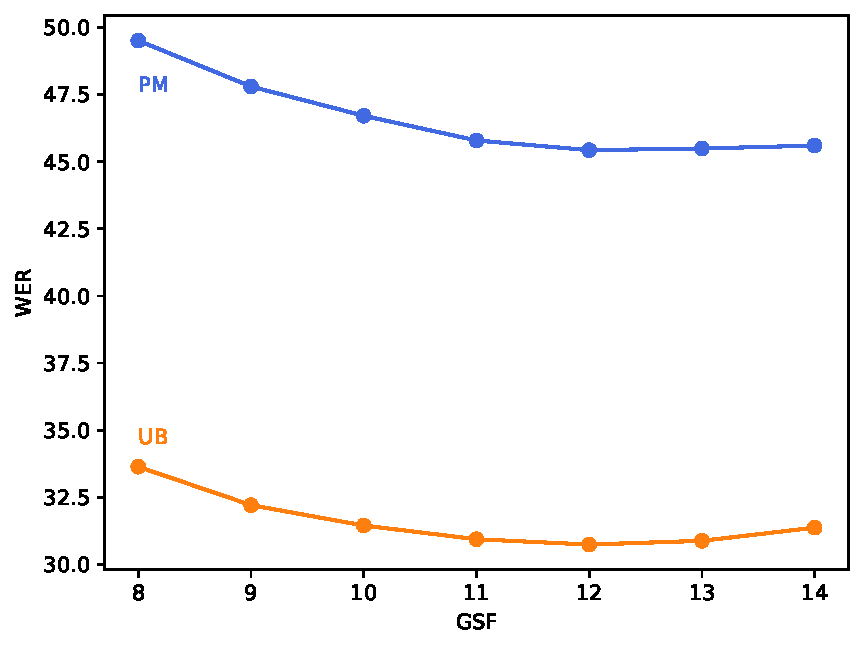
\includegraphics[width=0.5\textwidth]{figuras/gsf_gmm.pdf}
%    \caption{Resultats de l'exploració del valor GSF amb el model GMM-HMM i taules de look-ahead derivades del n-grama antic.}
%    \label{fig:gmm_wer}
%\end{figure}

%%%%%%%%%%%%%%%%%%%%%%%%%%%
%%%
%%%   Aliniament GMM-HMM
%%%

Finalment, vam usar l'eina \texttt{tLtask-align} amb el model GMM-HMM de 64 components, el \textit{lexicon}, la \textit{tlist}, els MFCCs i les transcripcions d'àudio per a obtenir els alineaments de senones a nivell de frame.
L'eina genera un fitxer d'eixida en el que s'indica, per a cada mostra d'entrenament, amb quins senones s'han alineat cadascun dels seus frames (vectors de característiques).




\subsection{FF-DNN-HMMs}
\label{cap05_am_dnn}
%%%%%%%%%%%%%%%%%%%%%%%%%%%
%%%
%%%   Entrenament DNN-HMM
%%%

El següent pas fou entrenar una FF-DNN per modelar $P(q_t|\textbf{x}_t)$ (veure Eq.~\ref{eq:cerca_nivell_paraules}) amb la informació dels alineaments calculats amb el model de GMMs. Per fer-ho, vam usar l'eina \texttt{tLdnn-train}. A continuació es detalla la configuració de la FF-DNN.
La capa d'entrada empra una finestra contextual de $\pm 5$ frames a esquerra i dreta del frame actual, es a dir, treballa amb vectors d'entrada de $11 \cdot 48 = 528$ components.
A continuació, sis capes ocultes de 2048 neurones amb activació per ReLu. Finalment, una capa d'eixida de 21589 unitats amb activació per softmax (tantes neurones com senones).
L'entrenament va requerir un temps d'execució total de 43 hores en una GeForce RTX 2080 Ti, al llarg de 20 èpoques, assolint un error de validació (FER) en \textit{development} de 56.1\%.
Si bé pot semblar una taxa d'error elevada, es tracta d'un valor acceptable, d'acord amb l'experiència  prèvia del grup MLLP-VRAIN. Alguns dels factors que justifiquen taxes FER elevades en aquest context són: en primer lloc, es tracta d'un problema de classificació complex, on hi ha que discriminar entre 21589 classes diferents. En segon lloc, les etiquetes de classe $q$ de totes les mostres d'entrenament, $(q, \textbf{x})$, proporcionades a la FF-DNN, han sigut generades per un model acústic generatiu, GMM-HMM, de baixes prestacions, pel que s'espera que una porció significativa de les etiquetes de classe siga incorrecta. Per últim, la funció d'error (FER) no considera l'existència d'etiquetes de classe (senones) similars. Per exemple, l'estat esquerre del trifonema \verb|l-a+o|, especialitzat en modelar la transició acústica del fonema \verb|/a/| al \verb|/l/|, i l'estat esquerre del trifonema \verb|k-a+o|, especialitzat en la transició del fonema \verb|/a/| al \verb|/k/|, són dues classes diferents, però pròximes entre elles i fàcilment confusibles. Però independentment del tipus d'error, FER sempre assigna error $= 1$ si l'etiqueta de classe no es exactament l'esperada, donant el mateix pes a errors greus que a errors assumibles.

Per tal de validar la correcció d'aquest model acústic, vam construir un segon sistema ASR temporal, conformat per aquest model acústic i la mateixa taula de look-ahead anterior. Amb aquest sistema, vam reconèixer automàticament el conjunt de \textit{development}, obtenint uns WERs de 29.0\% al corpus de PM i 23.0\% al corpus de UB.
Realitzant la comparació respecte al primer sistema, s'observa una millora notòria, assolint uns resultats potencialment prometedors. 

%\begin{figure}[!ht]
%    \centering
%    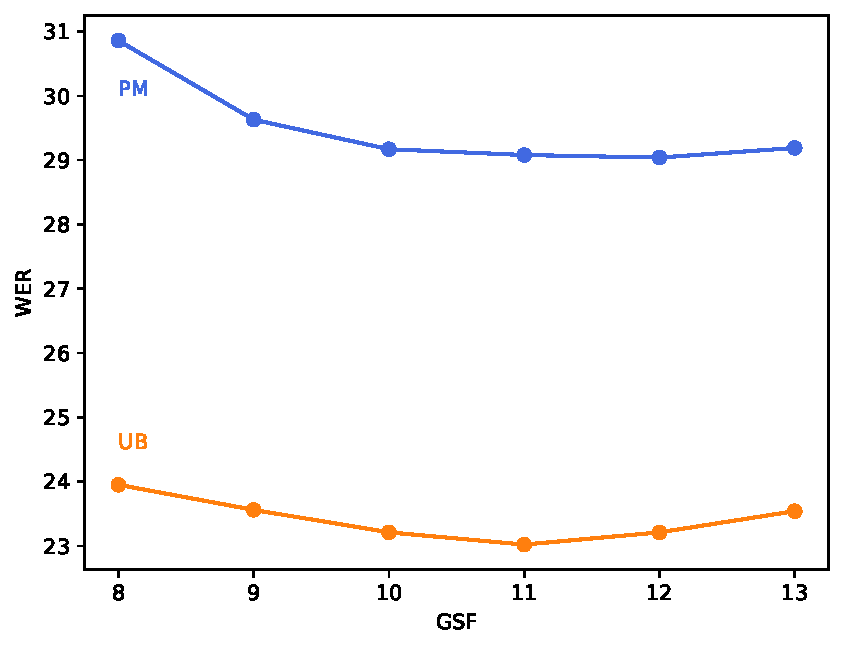
\includegraphics[width=0.5\textwidth]{figuras/gsf_dnn.pdf}
%    \caption{Resultats de l'exploració del valor GSF amb el model DNN-HMM i taules de look-ahead derivades del n-grama antic.}
%    \label{fig:dnn_wer}
%\end{figure}



%%%%%%%%%%%%%%%%%%%%%%%%%%%
%%%
%%%   Alineament DNN-HMM
%%%

Finalment, regenerarem els alineaments de senone a nivell de frame, usant la FF-DNN, amb l'objectiu d'obtenir una versió millorada d'aquests, similar a la millora observada en WER al conjunt de \textit{development} respecte al model GMM-HMM.




\subsection{BLSTM-HMMs}
\label{cap05_am_blstm}

%%%%%%%%%%%%%%%%%%%%%%%%%%%
%%%
%%%   Entrenament BLSTM-HMM
%%%

El pas final fou entrenar una xarxa BLSTM per modelar $P(q_t|\textbf{x}_t)$ amb la informació rebuda dels alineaments refinats, calculats pel model FF-DNN. Per fer-ho vam usar TensorFlow, mitjançant l'script \texttt{train\_blstm\_cudnn.py}. La configuració escollida de la BLSTM fou la següent.
S'utilitzaren 8 capes LSTM bidireccionals, cada una amb 512 neurones per a cada sentit temporal i, a l'igual com la FF-DNN, una capa d'eixida de 21589 neurones, tantes com senones.
Per a millorar la capacitat de generalització del model, es va aplicar la tècnica SpecAugment~\cite{park2019specaugment}, que consisteix en deformar les característiques d'entrada, emmascarar els blocs de canals de freqüència i emmascarar els blocs de passos de temps de forma aleatòria. Es realitzaren dues repeticions, amb màscares de 27 unitats d'ample horitzontal i 10 unitats d'ample vertical.

L'entrenament va requerir un temps d'execució total de 336 hores (aproximadament dues setmanes) emprant una GeForce RTX 1080, al llarg de 27 èpoques, assolint un error de validació (FER) mínim de 38.3\% sobre el conjunt de \textit{development}. La Figura~\ref{fig:wer_per_epoch} mostra l'evolució d'aquest error de validació en funció de les èpoques.
Comparant amb la FF-DNN, vam obtenir una reducció molt significativa del FER, de quasi 20 punts absoluts, demostrant, per una banda, la major capacitat d'aprenentatge d'aquest model, i d'altra banda, que els alineament refinats per la FF-DNN (les etiquetes de classe dels frames d'entrenament) són, efectivament, de major qualitat.

\begin{figure}[ht!]
    \centering
    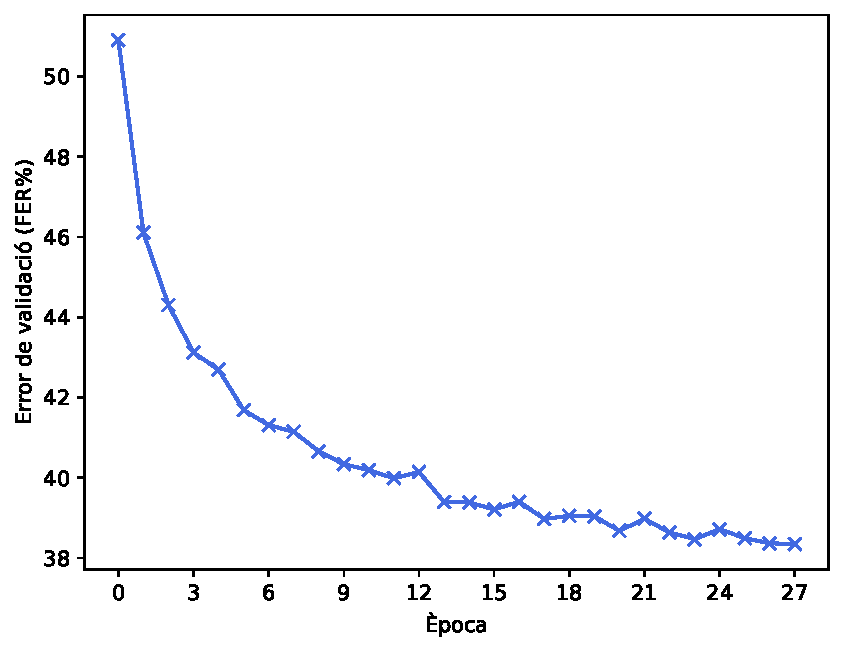
\includegraphics[width=0.6\textwidth]{figuras/validation_error.pdf}
    \caption{Error de validació en funció de les èpoques.}
    \label{fig:wer_per_epoch}
\end{figure}


\section{Construcció i optimització de sistemes ASR híbrids basats en BLSTM-HMM AMs}
\label{cap05_decod}
Una vegada entrenat el model acústic BLSTM-HMM, es procedeix a integrar-lo, juntament amb diferents models del llenguatge, en el descodificador híbrid de TLK per generar diferents sistemes ASR. Tots els LMs considerats en aquest treball han estat entrenats recentment per investigadors de l'MLLP, a excepció d'un model d'n-grames que prové del sistema ASR Francés de l'any 2017. A continuació es llisten i es donen els detalls més rellevants d'aquests LMs:

\begin{itemize}
    \item \textbf{n-grama (2017)}: model de 4-grames, provinent del sistema ASR Francés de 2017, entrenat amb totes les dades de text monolingüe descrites a la Secció~\ref{cap04_corpus_audio} (2.1G paraules), mitjançant el toolkit SRILM~\cite{srilm}. També es proporciona una versió superesporgada d'aquest model, convertida en taula estàtica de look-ahead per al descodificador.
    \item \textbf{n-grama}: model de 4-grames, entrenat amb totes les dades de text monolingüe (2.1G paraules), usant el toolkit KenLM~\cite{kenlm}. També es proporciona la taula estàtica de look-ahead corresponent.
    \item \textbf{TLM}: model de llenguatge neuronal basat en l'arquitectura Transformer, amb 24 capes Transformer, 512 neurones per capa, FF-DNNs de 4096 unitats, 12 \textit{attention heads}, i un \textit{embedding} de 768 dimensions, entrenat amb un subconjunt d'1G paraules amb el toolkit Fairseq~\cite{fairseq}.
    \item \textbf{n-grama + TLM}: interpolació lineal entre el 4-grama i el TLM, amb uns pesos òptims, calculats per al conjunt de development, de 40.7\% i 59.3\%, respectivament.
\end{itemize}

Per a la realització dels experiments, els valors dels LM look-ahead s'han calculat utilitzant un model molt esporgat derivat, en cada cas, del seu respectiu 4-grama. Al ser més menut, permet tindre precalculades totes les probabilitats en una taula i així accelerar la cerca. Així, quan en la cerca s'aplega a un node ``paraula'', la probabilitat d'aquest model menut es reemplaça per la del modl'original. Quan parlem d'emprar taules de look-ahead derivades d'un model, estarem parlant d'utilitzar directament les probabilitats d'aquest model esporgat.

Els sistemes ASR queden constituïts quan s'executa el descodificador de TLK mitjançant l'eina \texttt{tLtask-recognise}. Aquesta rep el model acústic (el model BLSTM-HMM), la taula de look-ahead estàtica, els vectors de característiques de les mostres a reconèixer i, opcionalment, un o més models del llenguatge externs, a banda dels valors dels diferents hiperparàmetres de descodificació.
D'aquests, destaquem els següents:

\begin{itemize}
    \item \textbf{GSF (Grammar Scale Factor)}, que escala el pes del model del llenguatge respecte al del model acústic durant la descodificació. 
    \item \textbf{PSF (Prior Scale Factor)}, que escala les probabilitats a priori, $P(q_t)$, dels HMM. 
    \item \textbf{LA (Grandària de la finestra, Look-Ahead)}, defineix el context futur, es a dir, el periode de temps, al que pot accedir la BLSTM per a buscar informació i emetre una possibilitat. És especialment útil quan tractem amb xarxes recurrents, ja que les permet considerar aquesta informació futura. Aquest paràmetre es necessari en un context d'streaming, ja que es la manera que tenim de limitar el futur necessari per a treballar.
    \item \textbf{LMHR (Language Model History Recombination)}, s'utilitza per a recombinar hipòtesis que utilitzen les mateixes últimes paraules a les seues histories. Força al descodificador a consolidar els prefixos de paraules i permetre una descodificació més ràpida, ja que la història del TLM no està limitada en longitud i ha de ser processada en cada iteració.
    \item \textbf{BEAM} representa la diferencia màxima que pot haver entre les puntuacions de l'objecte més probable i del menys probable. Així, si una hipòtesis es diferencia per un valor major al BEAM, es automàticament descartada. 
    \item \textbf{HP (Histogram pruning)}, defineix el nombre de històries màximes actives en cada instant.
    \item \textbf{LMHP (Language Model Histogram pruning)}, que controla el nombre d'històries noves que s'expandeixen a cada frame. Permet reduir el nombre de consultes al model del llenguatge.
\end{itemize}
En aquest cas, l'estudi dels paràmetres BEAM, HP i LMHP s'ha omès per restriccions temporals, sent valors fixes a BEAM$=160$, HP$=7500$ i LMHP$=60$, basats en coneixement previ del grup MLLP-VRAIN.

El primer sistema que vam estudiar utilitzava el model acústic BLSTM i les taules de look-ahead derivades del model d'n-grames de 2017.
Com que el LM era un cuatrigrama, l'LMHR no podia ser diferent de tres, en aquest i en posteriors experiments on sols intervé un 4-grama o una taula estàtica de look-ahead no es va explorar.
També s'ha estudiat l'impacte de la grandària de la finestra (lookahead), però no era significatiu, per tant, el seu valor va quedar fixat a $59$ frames al conjunt PM i $49$ frames al conjunt UB, tant en aquest com en posteriors experiments.
Finalment, es va estudiar el comportament davant de diferents valors del GSF i de PSF en funció del WER sobre el conjunt de \textit{development}. 
La Figura~\ref{fig:gsf_oldlm_small} mostra l'evolució del WER en funció del paràmetre GSF per a diferents valors de PSF.

\begin{figure}[ht!]
    \centering
    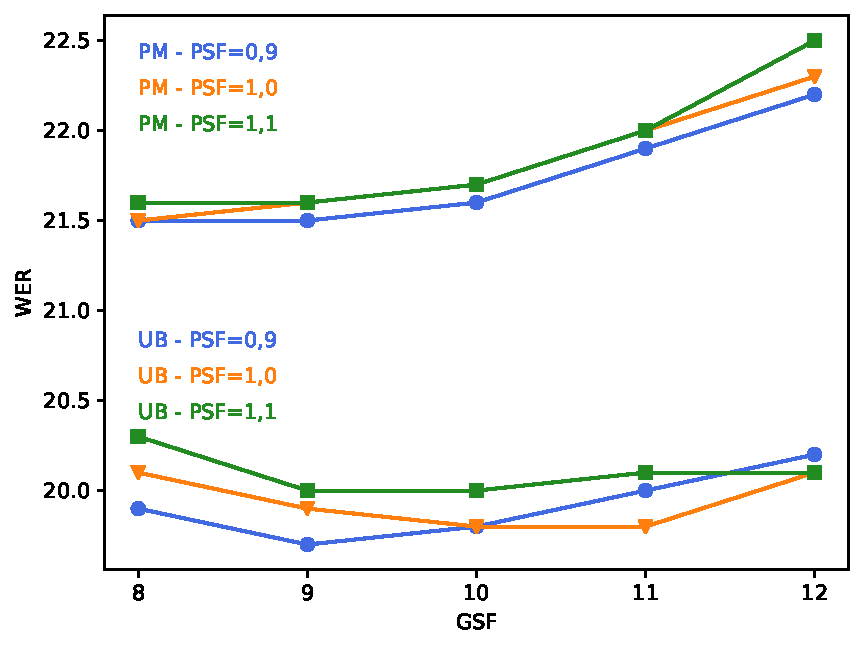
\includegraphics[width=0.5\textwidth]{figuras/gsf_oldlm_small.pdf}
    \caption{WER\%, calculat sobre els conjunts de \textit{development} de PM i UB, en funció dels paràmetres GSF i PSF amb el sistema format per el AM BLSTM i el LM basat en taules de look-ahead derivades del model del llenguatge de 2017. Es representen en diferents colors els valors de PSF per a ambdós corpus.}
    \label{fig:gsf_oldlm_small}
\end{figure}
Basant-se en les dades, el millor resultat per al conjunt PM, amb una WER de $21.5$\%, és el parell GSF=$8$ amb PSF= $1.0$ i GSF=$9$ amb PSF=$0.9$. Per a UB, el millor WER va ser $19.7$\%, per als valors de PSF=$0.9$ i GSF=$9$. Aquests valors de PSF van romandre fixos a la resta d'experiments, ja que no mostraven un gran impacte amb diferents valors.

En segon lloc, es va procedir a construir i optimitzar el sistema ASR resultant de combinar el nostre model acústic amb la taula de look-ahead estàtica i el LM de 4-grames de 2017.
En aquest cas es va optimitzar el GSF únicament, ja que el paràmetre LMHR encara necessitava estar fixat a tres.
La Figura~\ref{fig:gsf_oldlm_big} representa l'evolució del WER, calculat sobre els conjunts de \textit{development} de PM i UB, en funció del paràmetre GSF.

\begin{figure}[ht!]
    \centering
    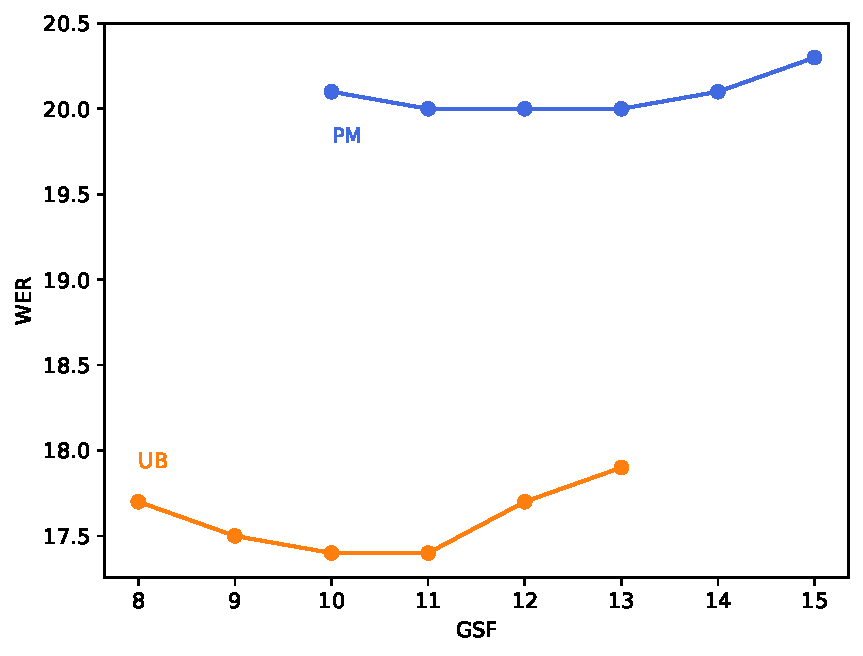
\includegraphics[width=0.5\textwidth]{figuras/gsf_oldlm_big.pdf}
    \caption{WER\%, calculat sobre els conjunts de \textit{development} de PM i UB, en funció del paràmetre GSF amb el sistema format pel AM BLSTM i el LM basat en taules de LA derivades del model del llenguatge de 2017 i el LM de 4-grames de 2017. Es representen en diferents colors els valors de PSF per a ambdós corpus.}
    \label{fig:gsf_oldlm_big}
\end{figure}
Obtinguérem unes puntuacions de WER de $20.5$\% per a PM, amb un GSF= $12$, i de $17.4$\% punts amb UB, amb un GSF=$10$. Veient aquests resultats es pot apreciar una millora respecte al model acústic antic, de $2$ punts de millora absoluta a PM i $0.9$ a UB.

En tercer lloc, estudiarem el comportament del nostre AM en conjunció dels nous LM de 4-grames.
En concret, vam portar a cap un primer experiment utilitzant sols la taula estàtica de look-ahead, i un segon que incorporava, a més, el model de 4-grames, explorant el GSF en cada cas.
La Figura~\ref{fig:gsf_newlm_sb} mostra els resultats d'ambdós experiments.

\begin{figure}[ht!]
    \centering
    \begin{subfigure}{0.45\textwidth}
        \centering
        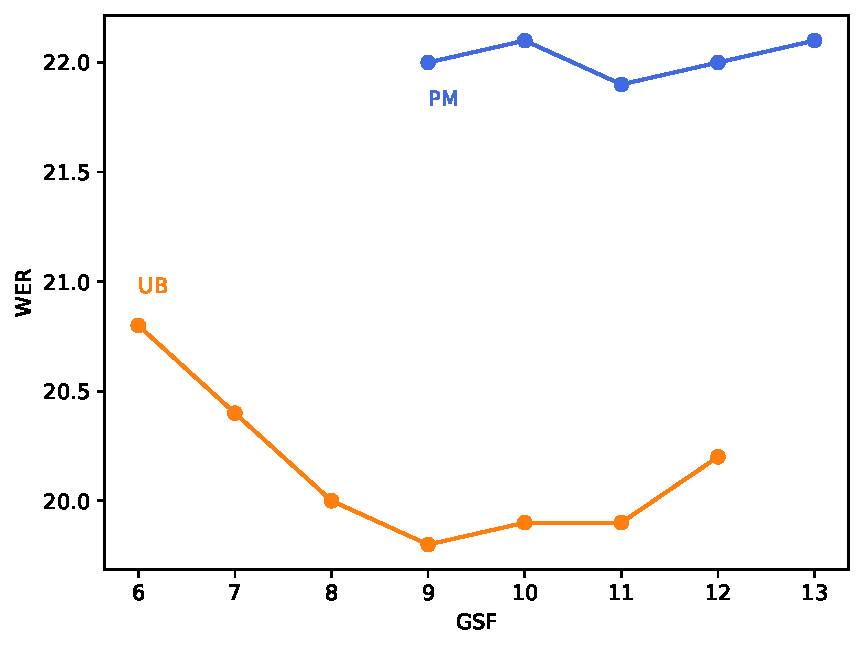
\includegraphics[width=\textwidth]{figuras/gsf_newlm_small.pdf}
        %\caption{Sistema amb taules de look-ahead basades en l'n-grama.}
    \end{subfigure}
    \begin{subfigure}{0.45\textwidth}
        \centering
        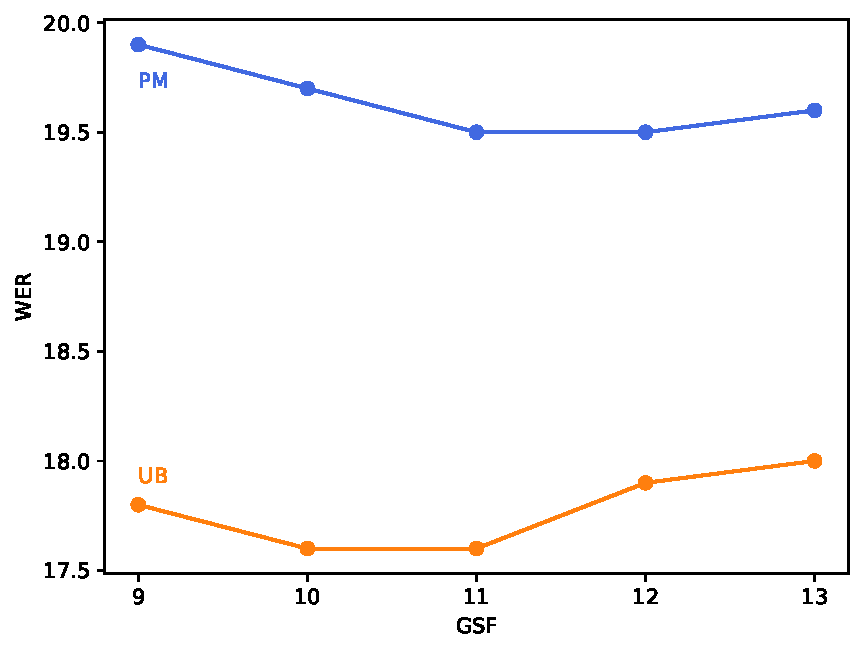
\includegraphics[width=\textwidth]{figuras/gsf_newlm_big.pdf}
        %\caption{Sistema amb taules de LA i l'n-grama nou.}
    \end{subfigure}
    \caption{WER\%, calculat sobre els conjunts de \textit{development} de PM i UB, en funció del paràmetre GSF; d'una banda (figura esquerra) per al sistema ASR que utilitza únicament les taules estàtiques de LA; i d'altra (figura dreta), per al sistema ASR que, a més, inclou el model de 4-grames.}
    \label{fig:gsf_newlm_sb}
\end{figure}

Pel que fa al model amb únicament taules de look-ahead, els millors resultats foren de $22.3$\% de WER a PM, amb GSF=$11$, i de $19.8$ punts a UB, amb GSF=$9$. Utilitzant també l'n-grama, les puntuacions milloraren fins a $20.1$\% en PM, amb GSF= $12$, i fins a $17.6$\% en UB, amb GSF= $11$.

En quart lloc, es va explorar la combinació del nostre AM amb el TLM. En un primer experiment fixarem el paràmetre LMHR $=9$ i explorarem els valors de GSF. La Figura~\ref{fig:gsf_newlm_tlm} mostra l'evolució del WER per als experiments, resultant que per a ambdós conjunts el millor valor fou GSF$=9$. Per aquesta raó, es va fixar a aquest valor i es va iniciar l'exploració de LMHR.

\begin{figure}[ht!]
    \centering
    \begin{subfigure}{0.45\textwidth}
        \centering
        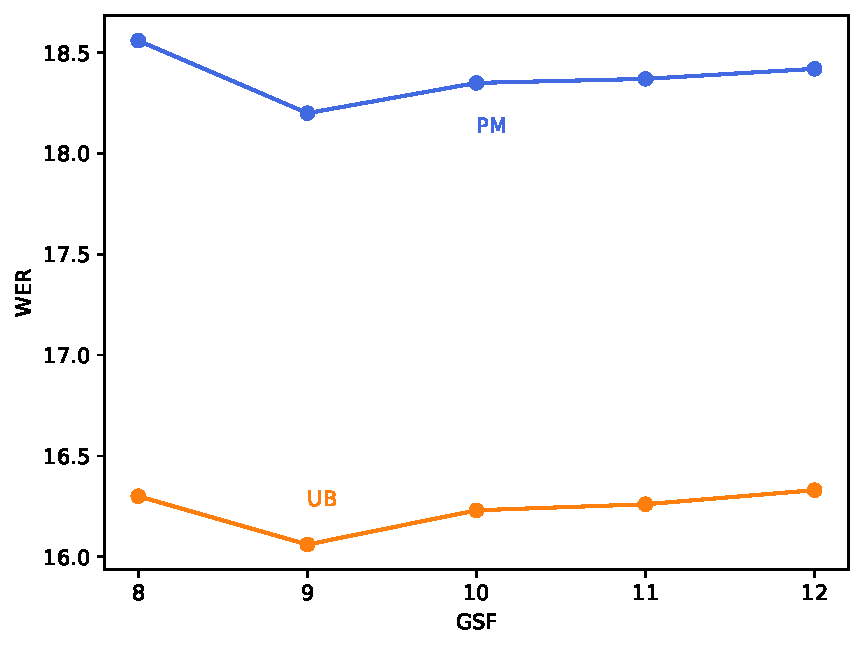
\includegraphics[width=\textwidth]{figuras/gsf_tlm.pdf}
    \end{subfigure}
    \begin{subfigure}{0.45\textwidth}
        \centering
        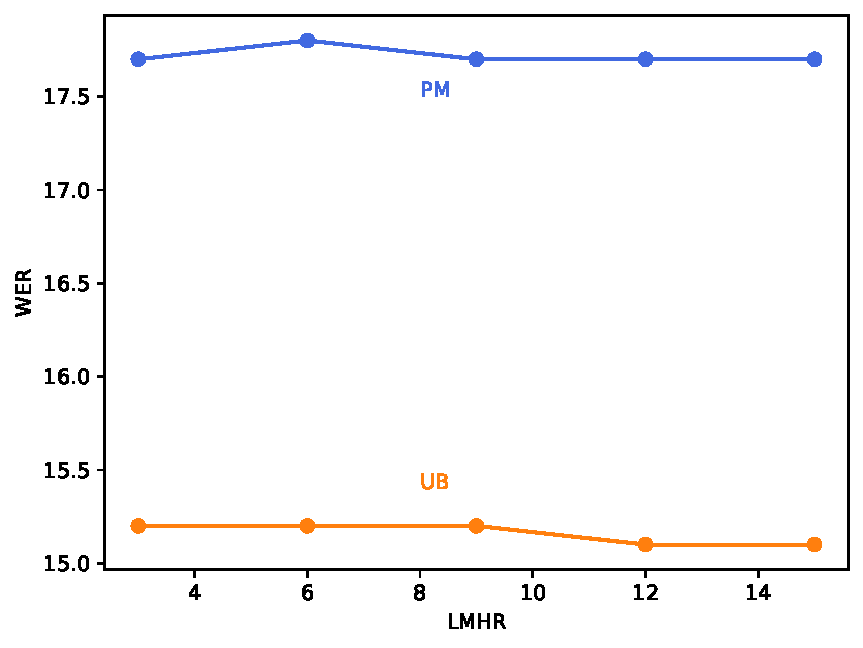
\includegraphics[width=\textwidth]{figuras/lmhr_tlm.pdf}
    \end{subfigure}
    \caption{}
    \caption{WER\%, calculat sobre els conjunts de \textit{development} de PM i UB per al sistema ASR que utilitza el TLM; d'una banda (figura esquerra) en funció del paràmetre GSF (fixant LMHR=3); i d'altra (figura dreta), en funció del paràmetre LMHR (fixant GSF=9).}
    \label{fig:gsf_newlm_tlm}
\end{figure}

Per una banda, s'obtingueren unes puntuacions WER de $18.4$\% per a PM, amb un LMHR de $9$, i de $16.0$\% per a UB, amb un LMHR de $9$. D'altra banda, el conjunt PM va obtindre una puntuació WER de $18.3$\% amb un LMHR de $6$, mentre que UB va obtindre una puntuació de $16.0$\% amb un LMHR de $12$.

Finalment, vam considerar el sistema que realitza una interpolació lineal entre l'n-grama i el TLM. El valor de LMHR va ser fixat al millor obtingut al pas anterior, ja que la mida mitjana de les frases al conjunt \textit{development} era d'aproximadament 10 paraules, i les variacions que podia aportar quedaven significantment reduïdes a costa del temps de còmput.
Els resultats poden observar-se a la Figura~\ref{fig:gsf_tlm_ngram}, aconseguint una WER en PM de $17.1$\% amb GSF$=11$, i de $15.2$\% amb GSF=$11$.

\begin{figure}[ht!]
    \centering
    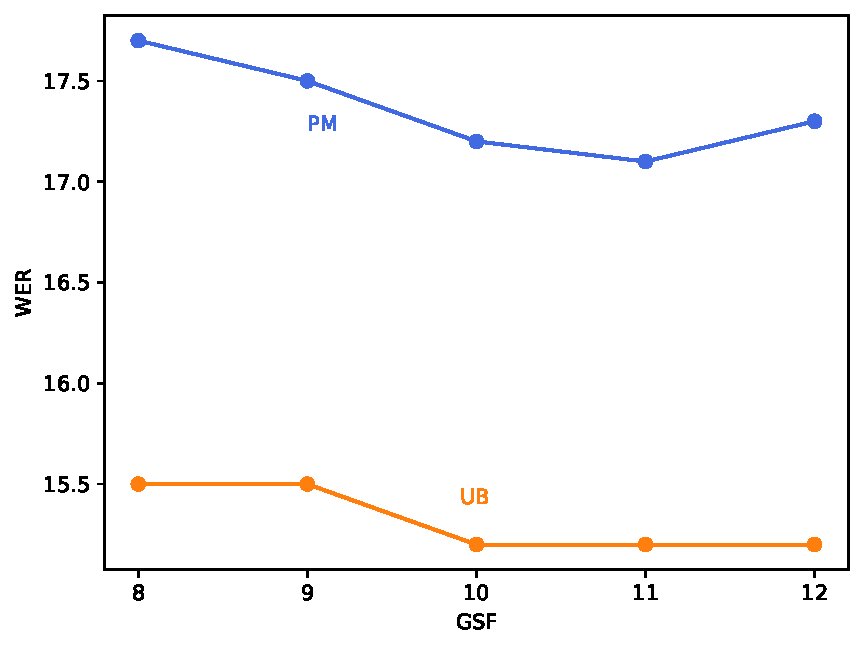
\includegraphics[width=0.5\textwidth]{figuras/gsf_tlm_ngram.pdf}
    \caption{WER\%, calculat sobre els conjunts de \textit{development} de PM i UB per al sistema ASR que utilitza l'interpolació lineal entre l'n-grama i el TLM en funció del paràmetre GSF.}
    \label{fig:gsf_tlm_ngram}
\end{figure}

\section{Avaluació i comparativa de sistemes ASR}
\label{cap05_aval}
En aquesta secció, primerament, es realitzarà l'avaluació final de tots els sistemes ASR considerats en el present treball, utilitzant els conjunts de \textit{test} de PM i UB. Després, els resultats de cada sistema es comparen amb els del sistema ASR Francés de 2017, per tal de mesurar l'efecte de les millores tecnològiques introduïdes.

El sistema ASR Francés de 2017 (d'ara endavant, sistema \textit{baseline}), és un sistema híbrid format per un model acústic FF-DNN-HMM amb activacions per ReLu, similar al model descrit al Capítol~\ref{cap03_dnnhmm}.
Aquest realitza, inicialment, un pas previ \guillemotleft Voice Activity Detection\guillemotright, que bàsicament es tracta de realitzar una segmentació d'on hi ha parla humana i on no per a únicament descodificar en aquests segments.
El procés de descodificació es realitza en dos passos. Un primer pas de reconeixement estàndard, i un segon pas amb \textit{fCMLLR (feature Constrained Maximum Likelihood Linear Regression)}, una tècnica que realitza una adaptació dels vectors de característiques a les locutores presents en les mostres, emprant les transcripcions automàtiques del primer pas de reconeixement com a referència.
Finalment, es realitza un tercer pas addicional, on és repuntuen les probabilitats del model del llenguatge amb un o diversos models del llenguatge externs més potents, en aquest cas, un 4-grama usat en els experiments de la Secció~\ref{cap05_decod}, i un model del llenguatge basat en RNNs.
El principal inconvenient d'aquest sistema és que, al ser multipassada, no està preparat per al reconeixement en streaming.
%Aquest sistema tenia les següents puntuacions WER: 22.1 i 19.0 punts per als corpus PM i UB al set \textit{dev} i 24.1 i 16.5 punts WER per als mateixos corpus al set \textit{test}.

Per altra banda, els sistemes ASR avaluats en aquest treball són aquells que acoblen el model BLSTM-HMM, amb la taula de look-ahead derivada del nou model d'n-grames, i diferents combinacions de models del llenguatge externs: 4-grama (2017), 4-grama, TLM i TLM interpolat amb 4-grama.
La taula~\ref{tab:resum_wer} resumeix les resultats WER, calculats sobre els conjunts de \textit{test} de PM i UB, amb tots els sistemes considerats en aquest estudi comparatiu.
També s'inclouen els millors resultats d'aquests sistemes en els respectius conjunts de \textit{development} (veure Secció~\ref{cap05_decod}).
%Les millores relatives del sistema BLSTM amb n-grama i Transformer respecte al sistema Baseline de 2017 són del 22.8\% al corpus de PM i del 15.6\% al corpus de UB.

\begin{table}[ht!]
    \centering
    \caption{WER\% dels diferents sistemes considerats en aquest estudi comparatiu, calculats sobre els conjunts de \textit{development} i \textit{test} dels corpus PM i UB. Els nostres sistemes estan representats de tal forma que els diferents LM proporcionats pel MLLP-VRAIN es combinen amb el AM desenvolupat en aquest treball.}
    \begin{tabular}{l|rr|rr}
                             & \multicolumn{2}{c|}{PM} & \multicolumn{2}{c}{UB} \\
        Sistema              & Dev        & Test       & Dev        & Test      \\ \hline
        Baseline (2017) & 22.1       & 24.1       & 19.1       & 17.3      \\
        BLSTM (+ taula LA)               & 22.3       & 22.2       & 20.7       & 19.0      \\
        \quad + n-grama (2017)       & 20.5       & 20.7       & 18.2       & 17.6      \\
        \quad + n-grama            & 20.1       & 20.2       & 18.4       & 17.4      \\
        \quad + TLM                & 17.7       & 18.9       & \textbf{15.1}       & 14.9      \\
        \qquad + n-grama  & \textbf{17.1} & \textbf{18.6} & 15.2  & \textbf{14.6}     
    \end{tabular}
    \label{tab:resum_wer}
\end{table}

Com pot observar-se, el sistema baseline és superat per tots els nostres sistemes ASR, excepte pel que únicament utilitza les taules de look-ahead, on obté un resultat pitjor en UB, però un poc millor en PM. Convé remarcar que el sistema de 2017 és un sistema multipassada que no està preparat per a funcionar en streaming. En canvi, els nous sistemes poden fer-ho.

També són rellevants les millores màximes, i és que quan es considera el TLM, s'obtenen unes millores absolutes de WER de fins a 5.5 punts, amb unes millores relatives del $22.8\%$ a PM i del $15.6\%$ a UB.

D'altra banda, convé ressaltar la comparativa entre el sistema baseline i el sistema BLSTM amb l'n-grama de 2017, ja que ens permet aproximar la millora que aporta el nostre model acústic al sistema final, a pesar que el sistema vell utilitzava un RNNLM que el nostre sistema no. Inclòs en aquest cas, s'assoleix una millora de les prestacions global, que arriba fins als 3.4 punts de diferència en el \textit{test} de PM, excepte en el \textit{test} d'UB, on el nostre sistema és lleugerament inferior en prestacions ($0.3$ punts WER). La nostra hipòtesi és que, en aquest cas concret, el model RNNLM marca la diferència, ajudant al sistema baseline a superar el nostre sistema.


% ---------------------------------------------------------------------
% ---------------------------------------------------------------------
% ---------------------------------------------------------------------

\chapter{Conclusions i treball futur}
\label{cap06__}

% ---------------------------------------------------------------------
% ---------------------------------------------------------------------
% ---------------------------------------------------------------------

En aquest treball s'ha descrit el procés de creació d'un model acústic d'avantguarda per a sistemes ASR Francés híbrids. Per aconseguir-ho, s'han emprat ferramentes software avançades i altament especialitzades com TLK i Tensorflow, així com un conjunt de dades d'entrenament de 663 hores de parla francesa transcrita manualment a un total de $6.8$ milions de paraules. 
El model acústic resultant, basat en Models Ocults de Markov amb les probabilitats d'emissió modelades per una xarxa neuronal recurrent de tipus BLSTM, ha estat combinat amb diferents models del llenguatge proporcionats per investigadors del grup de recerca MLLP-VRAIN, conformant potents sistemes ASR híbrids, aptes per funcionar en streaming.

Pel que fa al model acústic desenvolupat, el model BLSTM-HMM, podem concloure amb les dades experimentals que, aquest millora significativament el model acústic multipassada del sistema baseline, aportant millores relatives de WER de fins a un 16.2\% en el conjunt de \textit{test} PoliMèdia.

El millor sistema ha estat aquell que combina el nostre BLSTM-HMM AM amb una interpolació lineal d'un model de 4-grames i un Transformer LM, obtenint millores, respecte al sistema baseline, de 2.7 punts WER en UB i de 5.5 punts en PM, és a dir, entre un 15.6\% i un 22.8\% de millora relativa en funció de la tasca. A més, convé ressaltar que aquest sistema està preparat per treballar en entorns d'streaming, al contrari del sistema baseline.

Aquest treball ha deixat portes obertes a molt de treball futur:
\begin{enumerate}
    \item Realitzar una exploració dels paràmetres per ajustar la latència del sistema per al seu ús en streaming.
    \item Generar una imatge docker amb el millor sistema ASR per facilitar el seu desplegament al CERN.
    \item Exploració niada dels hiperparàmetres de descodificació que s'han deixat fixes per restriccions temporals.
    \item Ampliar el conjunt d'entrenament de dades acústiques transcrites, doncs 663 hores són poques per als actuals estàndards de la literatura (milers d'hores d'entrenament).
    \item Recopilar conjunts de dades de \textit{dev} i \textit{test} específics del CERN, per avaluar els sistemes ASR amb dades representatives dels continguts audiovisuals que es generen en aquesta institució.
    \item Explorar noves topologies BLSTM i Transformer. 
\end{enumerate}




% -------------------------------------------------------
% -------------------------------------------------------
% -------------------------------------------------------
% Bibliografía

\bibitemsep = 3ex
\bibhang = 2em

\printbibliography[heading=bibintoc,title=\bibname]


% -------------------------------------------------------
% Índice alfabético

\cleardoublepage
\phantomsection
\addcontentsline{toc}{chapter}{\indexname}

\printindex

% -------------------------------------------------------
% Fin del documento

\end{document}

% ---------------------------------------------------------------------
% ---------------------------------------------------------------------
% ---------------------------------------------------------------------
